\documentclass[final,3p,times,twocolumn]{elsarticle}
\usepackage{amssymb}
\usepackage[fleqn]{amsmath}
\usepackage{graphicx}
\usepackage{footnote}
\usepackage{graphicx}
\usepackage{array,booktabs}
\usepackage{algorithmic,algorithm}
\usepackage{pbox}
\usepackage{enumitem}
\usepackage{color}
\usepackage{hyperref}
\setlength\parskip{\baselineskip}
%\setlength{mathindent}{0pt}
\setlength\parindent{0pt}
\journal{MPhil in Scientific Computing}

\begin{document}

\begin{frontmatter}

\title{Analyzing the Higgs signal using Support Vector Machines}
\author{Vidhi Lalchand}
\address{Cavendish Laboratory, Department of Physics, J J Thomson Avenue, Cambridge. CB3 0HE}

\begin{abstract}
This paper examines the use of Support Vector Machines (SVM) as a machine learning tool for classifying the outcomes of atomic collisions. We demostrate the SVM approach on a simulated dataset provided by ATLAS physicists which relates to the popular case of the Higgs Boson. The dataset has labelled samples belonging to two classes -- `signal' and `background'. The `signal' class represents collisions that indicate the presence of a Higgs particle and the `background' class represents collisions that result in the creation of particles which are uninteresting from a Higgs perspective. We demonstrate the feasibility of SVMs in this supervised binary classification task. We show that hyper-parameter tuning combined with pruning of the training dataset are highly efficient ways to prepare an SVM for this task. The performance of the classifier in this context is assessed on the basis of a physics motivated metric called the \textit{Approximate Median Significance} score (AMS for short). The final solution attains an AMS score of 3.38. The highest reported AMS score on this dataset is 3.8.
\end{abstract}
\end{frontmatter}

\section{Background}

In 2012, the ATLAS\footnote{A Toroidal LHC Apparatus} and the CMS\footnote{Compact Muon Solenoid} experiment observed a new particle in the proton-proton collisions at the LHC (Large Hadron Collider) in CERN. The discovery had a statistical significance of 5$\sigma$ (five-sigma). Five-sigma corresponds to a p-value of $3*10^-7$, or a 1 in 3.5 million chance that the results obtained were purely due to chance. In essence, 5$\sigma$ denotes a high confidence in the results obtained. The particle, the Higgs boson, was postulated nearly five decades ago within the framework of the Standard Model (SM) of particle physics. The existence of this particle provides support to the theory that a field permeates the universe through which fundamental particles acquire mass, a theory which is cardinal for the completeness of the Standard Model. The proton-proton collisions in the ATLAS detector produce thousands of collision events per second. Each collision event is summarised by numeric information represented by a vector of several dimensions. These represent the features, as in standard machine learning applications. CERN have made publicly available a simulated dataset  mimicking the challenges of real collision data. This dataset was used by ATLAS physicists in designing statistical tools that could aid in search of collisions that indicate the presence of a Higgs. The goal of this project is to cast this challenge as a supervised binary classification problem. The classification task is to classify collisions which represent the Higgs signal from those that represent background. 

In order to promote collaboration between high energy physicists and machine learning experts a challenge (HiggsML challenge for short) was organized by a small group of ATLAS physicists. It was hosted by Kaggle at  
\url{https://www.kaggle.com/c/higgs-boson} from May to September 2014. The simulated dataset used in this paper was released to the participants for training. The immediate goal of the challenge was \textit{to explore the potential of advanced classification methods to improve the statistical significance of the experiment}\cite{RM}. 

Although the SVM approach is widely used in binary classification tasks, there are no articles examining the use of SVMs on the Higgs dataset. The winning solution of the HiggsML challenge comprised of an ensemble of multi-layer feed-forward neural networks, the networks used a set of identical fine-tuned parameters and only differed  only in their initialization training sets \cite{Gabor}. Other techniques that were popular among participants were variants of boosted decision trees. 

After an introduction to the physics goal of the problem in Section \ref{physics}, the machine learning set-up is described in Section \ref{MLC}. Section \ref{ams} and Section \ref{performance} are particularly important as they introduce a  statistical set-up for quantifying performance of classifiers in the context of the problem. Section \ref{SVM} introduces the mathematical framework for SVMs and Section \ref{learning_pipe} describes the implementation details of the SVM algorithm in the context of the classification problem. The results are  summarised in Section \ref{conclusion}.

\section{Physics Motivation}
\label{physics}
Many particles produced in the proton-proton collisions are unstable and decay almost instantaneously into other particles. These particles decay further to more stable final state particles. These sets of second order and third order particles represent a \textit{decay channel} or a \textit{decay product}. The Higgs boson $(H)$ is unstable and is observed to have 5 main experimentally accessible decay channels. Each occurs which a certain probability, this is called the branching ratio. The branching ratios of the Higgs boson depend on its mass and are precisely predicted in the standard model. For a SM Higgs of mass 125 Gev, the first-order decay products and their respective probabilities are : 

\scalebox{0.7}{
\begin{tabular}{|l|l|l|}
\hline
\rule[-1ex]{0pt}{2.5ex} Decay Channel & Description & Branching Ratio \\ 
\hline 
\rule[-1ex]{0pt}{2.5ex}  $H \rightarrow b\bar{b}$ & b quark and its anti-quark & 0.58 \\ 
\rule[-1ex]{0pt}{2.5ex} $ H \rightarrow \tau^{+} \tau^{-} $ & $\tau$ lepton and its anti-particle & 0.064 \\ 
\rule[-1ex]{0pt}{2.5ex} $ H \rightarrow \gamma\gamma $ & di-photon channel & 0.0023 \\ 
\rule[-1ex]{0pt}{2.5ex} $ H \rightarrow W^{+}W^{-} $ & W boson and its anti-particle & 0.14 \\ 
\rule[-1ex]{0pt}{2.5ex} $ H \rightarrow Z^{0}Z^{0} $ & 2 Z bosons &  0.016\\
\hline
\end{tabular}} 

This paper focuses on the  $H \rightarrow \tau^{+} \tau^{-}$ decay channel where the signal events indicate a Higgs decay to two taus and background events are characterized by the same tau-tau channel but from decay of a non-Higgs particle, fig. \ref{H_decay}.  
 
Several of the particles produced in the first order decay, decay instantaneously into a cascade of lighter particles. The surviving particles which live long enough for their properties to be measured by the detector are called \textit{final-state} particles. The different types of particles and pseudo-particles \footnote{explain pseudo-particles.} recorded in the final state of collisions in the dataset are electrons ($e$), muons ($\mu$), hadronic taus, jets and missing transverse momentum. These are explained below. 

\subsection{Fundamental and Other particles}

Electrons ($e$), muons ($\mu$) and the tau lepton ($\tau$) are the three leptons from the standard model. They are \textit{elementary}\footnote{An elementary particle is a particle whose substructure is unknown} particles. Neutrinos are elementary particles that belong to the lepton family but with a mass that is tiny compared to other leptons. Neutrinos produced in the decay escape detection completely 

\textit{Hadrons} are composite particles made up of quarks and/or antiquarks that are held together by gluons. The proton is a hadron. When two protons collide, they create a spray of hadrons. \textit{Jets} can be thought of as an ensemble of hadrons that are created when quarks and gluons try to escape in energetic proton-proton collisions. Jets are pseudo particles rather than real particles, they appear in the final state as a collimated energy deposits with charged tracks \cite{CMS:2} \cite{RM}. 

Properties of electrons and muons that appear in the final state are measured directly in the detector. Taus, on the other hand decay immediately after their creation into either, an electron and two electron neutrinos, a muon and two muon neutrinos or a bunch of hadrons (called the hadronic tau) and one tau neutrino. 

The three dominant channels of tau decay :

\begin{enumerate}[noitemsep]
\item{$\tau \rightarrow e^{-}\nu_{e}\nu_{e}$} [an electron and two neutrinos]
\item{$\tau \rightarrow \mu^{-}\nu_{\mu}\nu_{\mu}$} [a muon and two neutrinos]
\item{$\tau \rightarrow$  $\tau$-hadron and $\nu_{\tau}$ [a tau-hadron and a neutrino]}
\end{enumerate} 

In the dataset provided, the final state consists of a specific topology :

\begin{enumerate}[noitemsep]
\item A lepton (we do not know if the lepton is a muon or an electron)
\item A hadronic tau 
\item Neutrinos 
\end{enumerate}

Apart from these jets appear in the final state and we have the measured properties of the \textit{leading} and \textit{sub-leading} jet. The leading jet has a higher transverse momentum than the sub-leading jet. 

\subsection{Properties of final-state particles}

The ATLAS detector measures three properties of each of the detectable final state particles, they are :

\begin{enumerate}[noitemsep]
\item{The \textit{type} (lepton, hadronic tau, jets)} \item{The \textit{energy}, $E$}
\item{The \textit{3D direction} expressed as a vector $(p_{x}, p_{y}, p_{z})$}
\end{enumerate}

\textit{Note:} Neutrinos are not among the detected final-state particles but appear in the final state. The feature associated with the undetected neutrinos is the \textit{missing transverse momentum}. This deserves a detailed explanation which is provided in the section below.

\subsection{Missing transverse momentum}
\label{missing}

In the 3D reference frame of ATLAS, the $z$-axis points along the horizontal beam line. The $x-y$ plane is perpendicular to the beam axis and is called the \textit{transverse plane}. The transverse momentum is the momentum of an object transverse to the beam axis (or in the transverse plane). The law of conservation momentum promotes the idea of \textit{missing transverse momentum}.

The law of conservation momentum states that the total momentum is conserved in a closed system before and after a collision. We do know that the initial momentum in the plane transverse to the beam axis is zero. Hence, the sum of transverse momentum of all particles (detected + undetected) post-collision should be zero. 

The missing transverse momentum is defined as, $E_{miss}^{T} =  - \sum_{i} \vec{p_{T}}(i) $ for visible particles $i$ where $\vec{p_{T}}$ is the transverse momentum. Essentially, a net momentum of outgoing visible particles indicates missing transverse momentum attributed to particles invisible to the detector, like neutrinos. We know that the final state events consists of neutrinos and it is reasonable to estimate that they make up a lot of the missing transverse momentum.

\subsection {Physics goal} 

Based on the properties of the decayed products, the parent particle (Higgs or non-Higgs) is to be identified. \cite{RM}

Detection of a Higgs particle requires inferring its known mass (125GeV) from the total momentum of all its decay products (See \ref{AppA} for the mathematical description of the invariant mass principle). However, this mass reconstruction process might not always be possible due to, 

\begin{enumerate}
\item{The presence of particles (like neutrinos) in the final state which escape detection and their properties cannot be measured.}
\item{Particles like the Z-boson which have decay signatures very similar to the Higgs and occur a lot more frequently than the Higgs.}
\end{enumerate}
 
In the section below we elaborate on these points which explain what makes the Higgs classification a challenging machine learning problem.

\subsection{\texorpdfstring{$ H \rightarrow \tau^{+} \tau^{-} ${c}}channel}
\label{H-TT}

We narrow our focus to the tau-tau decay channel of the Higgs. In the simulated dataset, the positive (signal) class represent events in which the Higgs Boson decays into two taus. The exploration of this specific decay channel is challenging due to the following reasons. 

\begin{itemize}

\item{The decay into two taus is not a unique channel, in fact the Z boson can also decay into two taus, further this happens a lot more frequently than the Higgs. The precise mass of the Z boson is 91 GeV, since this is not very far from the mass of the target Higgs (125 GeV), the two decays produce events which have very similar signatures and this prevents a clean separation of the parent candidate.}

\begin{figure}
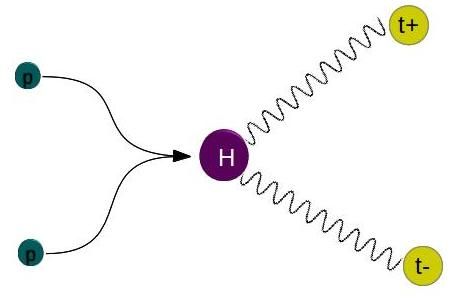
\includegraphics[scale=0.5]{Images/H1.jpg}
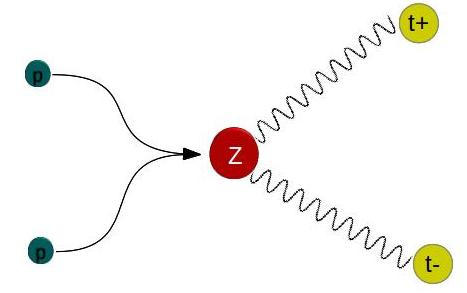
\includegraphics[scale=0.5]{Images/Zb.jpg}
\caption{The Higgs (H) and Z-boson decaying to two taus}
\label{H_decay}
\end{figure}

\item{Taus are heavy and unstable, they decay instantaneously. Their dominant decay modes involve neutrinos and the presence of these undetectable particles in their decay make it difficult to reconstruct the mass of the Higgs on an event by event basis.}
\end{itemize}

\begin{figure}
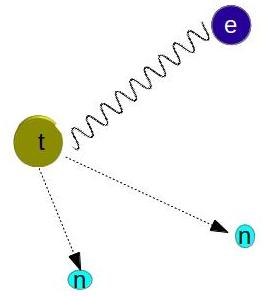
\includegraphics[scale=0.5]{Images/Te.jpg}
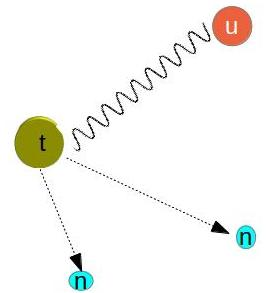
\includegraphics[scale=0.5]{Images/Tm.jpg}
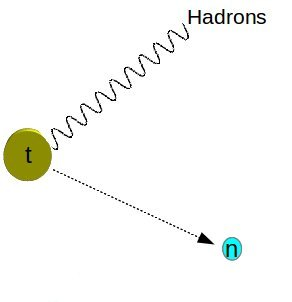
\includegraphics[scale=0.4]{Images/Th.jpg}
\caption{The tau decay to an (i) electron and 2 neutrinos, (ii) muon and 2 neutrinos, (iii) hadrons and a neutrino}
\label{Tau_decay}
\end{figure}

\subsection{A Note on the Higgs Mass}

The mass of the Higgs boson does not directly fall out of the standard model. In 2011 data collected by the CMS allowed a first thorough investigation into the existence of the SM Higgs over a wide mass range. The experiment yielded a first cut excluding the Higgs mass in the range of 127-600 GeV. This left a narrow window where a low-mass Higgs could still exist. In the region below 127 GeV the analysis showed a signal in the vicinity of 124 GeV, however, more data would be required to resolve the precise mass and reach a statistical significance of around 5$\sigma$. The LHC operation at 8 TeV in 2012 coupled with improved statistical analysis revealed an excess of events resolving to a particle with a mass of 125 GeV and this was agreed upon by the collaboration. 

\section{Machine Learning Challenge}
\label{MLC}
Both background and signal events in our dataset have the same topology,  they are tau-tau events where one tau decays into a lepton (electron or a muon) and 2 neutrinos and the other tau decays into hadrons and a neutrino. Additionally, properties of jets which originate from a high energy quark are measured by the detector.

Parent (Higgs / Non-Higgs) $\rightarrow$ $\tau^{-}\tau^{+}$ $\rightarrow$ lepton ($e^{-}$ or $\mu^{-}$) + Hadronic-tau + (Neutrinos) + Jets
 
The signal events represent collisions where the parent Higgs was created and background events represent collisions where the parent particle was not Higgs but shared the same tau-tau decay channel. The neutrinos are in parentheses to denote that their properties are not measured. The only feature pertaining to the neutrinos is the missing transverse momentum explained in Section \ref{missing}.

\subsection{The Dataset}

The signal events in the dataset have a class label 1 and background events have class label 0. The training set consists of 250,000 rows, each row denotes a collision event. The columns represent features which would serve as inputs to the classifier. The primary features are described in \ref{features}. Each row has a non-negative weight which corrects for the mismatch between the natural probability of a signal event and the probability applied by the simulator. The importance weights are not given as inputs to the classifier as the weight distribution of the signal and background events are very different and this would give away the class label immediately. The probability of a signal event in the natural world is several magnitudes lower than that of a background event. The signal and background events in the simulated dataset  are re-normalized to produce a more balanced classification problem where the ratio of signal to background events is close to 30 : 70. While the weights are not used as inputs they are used in assessing the performance of classifiers \cite{CMS:1}.

\subsection{Features}
\label{features}

The primary features in the dataset comprise of 3 measured properties of each of the detectable final-state particles and pseudo-particles. The measured properties are :

\begin{itemize}[noitemsep]
\item Pseudorapidity 
\item{Azhimuth angle} 
\item{Transverse momentum}
\end{itemize}

The final-state particles and pseudo-particles are :

\begin{enumerate}[noitemsep]
\item{Hadronic-tau} 
\item{Lepton} 
\item{Leading Jet}
\item{Sub-leading Jet}
\end{enumerate}

A full description of the physical meaning of each of the measured properties is in \ref{Pfeatures} The list of primary features, as in \cite{RM} :

\begin{enumerate}[noitemsep]
\item{\textbf{PRI$\_$tau$\_$pt} The transverse momentum $\sqrt{p_{x}^2 + p_{y}^2}$ of the hadronic tau.}
\item{\textbf{PRI$\_$tau$\_$eta} The pseudorapidity $\eta$ of the hadronic tau.}
\item{\textbf{PRI$\_$tau$\_$phi} The azhimuth angle of the hadronic tau.}
\item{\textbf{PRI$\_$lep$\_$pt} The transverse momentum $\sqrt{p_{x}^2 + p_{y}^2}$ of the lepton (the type of lepton whether electron or muon is not known).}
\item{\textbf{PRI$\_$lep$\_$eta} The pseudorapidity $\eta$ of the lepton.}
\item{\textbf{PRI$\_$lep$\_$phi} The azhimuth angle $\phi$ of the lepton.}
\item{\textbf{PRI$\_$met} The missing transverse momentum $E_{miss}^{T}$.}
\item{\textbf{PRI$\_$met$\_$sumet} The total transverse energy in the detector.}
\item{\textbf{PRI$\_$met$\_$phi} The azhimuth angle $\phi$ of the missing transverse energy.}
\item{\textbf{PRI$\_$jet$\_$num} The number of jets, either 0, 1, 2 or 3.}
\item{\textbf{PRI$\_$jet$\_$leading$\_$pt} The transverse momentum $\sqrt{p_{x}^2 + p_{y}^2}$ of the leading jet.}
\item{\textbf{PRI$\_$jet$\_$leading$\_$eta} The pseudorapidity $\eta$ of the leading jet.}
\item{\textbf{PRI$\_$jet$\_$leading$\_$phi} The azhimuth angle $\phi$ of the leading jet.}
\item{\textbf{PRI$\_$jet$\_$subleading$\_$pt} The transverse momentum $\sqrt{p_{x}^2 + p_{y}^2}$ of the sub-leading jet.}
\item{\textbf{PRI$\_$jet$\_$subleading$\_$eta} The pseudorapidity $\eta$ of the sub-leading jet.}
\item{\textbf{PRI$\_$jet$\_$subleading$\_$phi} The azhimuth angle $\phi$ of the sub-leading jet.}
\item{\textbf{PRI$\_$jet$\_$all$\_$pt} The scalar sum of the transverse momentum of all the jets of the events.}
\end{enumerate}

Apart from these there are 13 derived features, most of them are computed by operations on primary features. For example, feature \textbf{DER\_pt\_h} is the vector sum of the transverse momentum of the hadronic tau, the lepton, and the missing transverse momentum. 
  
\subsection{The formal problem}
\label{math}

The description in this section is based on Section 4.1 of \citep{RM}.
Let $\mathcal{D} = \{(\mathbf{x}_{1},y_{1},w_{1}),...(\mathbf{x}_{n},y_{n},w_{n}) \}$ be the sample data set provided by ATLAS,     $\mathbf{x}_{i} \in \mathbb{R}^d$ is a \textit{d}-dimensional feature vector, $\textit{y}_{i} \in \{b,s\}$ is the class label and $\textit{w}_{i} \in \mathbb{R}^{+}$ is a non-negative weight associated with each sample. Let $\mathcal{S} = \{i : y_{i} = s\}$ and $\mathcal{B} = \{i : y_{i} = b\}$ represent index sets of signal and background events respectively. Also, $n_{s} = |\mathcal{S}|$ and $n_{b} = |\mathcal{B}|$ represent the number of signal and background events in the dataset. 

It is important to clarify the role of the weights associated with each sample in the training dataset. The simulated dataset differs from the real-world dataset in the frequency with which signal events occur. The fraction $n_{s}/n_{b}$ is not reflective of the proportion of the prior class probabilities $P(y = s)/P(y = b)$, this is because $P(y = s) \ll P(y = b)$ and the true distribution of events in the dataset would yield an extremely unbalanced classification problem with $n_{s}$ significantly lower than $n_{b}$.  In order to correct for this bias, all events are weighted with importance weights reflecting their true probability of occurrence.

In each class, the quantities $N_{s}$ and $N_{b}$ are defined as, 
\begin{equation}
\sum_{i \in \mathcal{S}} w_{i} = N_{s} \hspace{5mm} 
\textrm{ and } \hspace{5mm} 
\sum_{i \in \mathcal{B}} w_{i} = N_{b} 
\label{weights}
\end{equation}

These constants have physical meaning, they are the expected total number of signal and background events during the time interval over which the data has been recorded (in the dataset used, it is the year 2012).

The objective function that the classifier is trained to optimise (described in Section \ref{ams}) depends on the \textit{unnormalized} sum of weights to make the set-up invariant to the number of simulated signal and background events.

Let $ h : \mathbb{R}^{d} \rightarrow \{b,s\} $ be an arbitrary binary classifier. The selection region $\mathcal{H} = \{\textbf{x} : h(\textbf{x}) = s\}$, $\textbf{x} \in \mathbb{R}^{d}$ is the set of points classified by $h$ as a signal, these are the \textit{predicted} positives. Let $\hat{\mathcal{H}}$ denote the index set of points that $h$ classifies as signal, $$ \hat{\mathcal{H}} = \{i : \textbf{x}_{i} \in \mathcal{H}\} = \{i : h(\textbf{x}) = s \}  $$

The quantities, 
\begin{equation} 
s = \sum_{i \in \mathcal{S}\cap \hat{\mathcal{H}}} w_{i} \hspace{5mm}
\textrm{    and    } \hspace{5mm}
b =\sum_{i \in \mathcal{B}\cap\hat{\mathcal{H}}} w_{i} 
\label{unbiased}
\end{equation} 

are unbiased estimators of the expected number of signal and background events selected by the classifier $h$ as signals. $s$ and $b$ are true positive and false positive rates.  

The binary classifier $ h : \mathbb{R}^{d} \rightarrow \{b,s\} $ calculates a discriminant value $f(\textbf{x}) \in \mathbb{R},\textbf{x} \in \mathbb{R}^{d}$ which is a score giving small values for the negative class (background) and large values for the positive class (signal). One puts a threshold of choice $\theta$, on the discriminant score and classifies all samples below the threshold as belonging to the negative class ($b$) and all samples with a score above the threshold as belonging to the positive class ($s$). 

The discriminant function $f(\textbf{x})$, also called \textit{decision function}, is evolved at the time of training and applied to test samples to reach classification decisions.

Most classifiers are optimized to improve classification accuracy on a held-out test set. The classification accuracy is the fraction of correctly classified samples belonging to all classes. Using the terminology \textit{TP} : True positives, \textit{TN} : True negatives, \textit{P} : Positives and \textit{N} : Negatives, the classification accuracy is defined as 
the fraction $\frac{\displaystyle TP + TN}{\displaystyle P + N}$. In the context of our problem a metric such as the overall classification accuracy is a weak indicator of the performance of a classifier. This is because the class distributions are skewed rather than balanced. Given that around 70\% of the samples belong to the negative class, a classifier that assigns each sample to the negative class will have an accuracy score of 70\%, but this largely ignores the strength of the classifier in classifying samples of the positive class correctly. 

In many contexts the question surrounding reliable performance measurement is tied to the problem at hand. For instance, in bioinformatics, the significance of a discovery is tied to whether the false discovery rate, defined as, $\frac{\displaystyle FP}{\displaystyle FP+TP}$ (where FP : False positive and TP : True Positive) is small enough. 

In a similar spirit, the physicists at ATLAS specify an objective function to be maximized by the classifier. It is called the \textit{Approximate Median Significance} metric. The section below elaborates on the statistical motivation for its definition.

\subsection{Approximate Median Significance (AMS) Metric}
\label{ams}

The AMS is an objective function that is applied on the set of points in a region of the feature space where an excess of signal events is expected over background. This is the \textit{selection} region $\mathcal{H}$. The selection region is defined by the value of the cut-off. For a given classifier $h$ with a discriminant function $f(\textbf{x})$ for $\textbf{x} \in \mathbb{R}^d$ and cut-off value $\theta$ the selection region is defined by, $ \mathcal{H} = \{\textbf{x} : f(\textbf{x}) > \theta \}$.

The total number of events $(n)$ in the selection region of a classifier $h$ can be partitioned into two groups :

\begin{itemize}
\item{Selected Background events : \begin{displaymath} b =\sum_{i \in \mathcal{B}\cap\hat{\mathcal{H}}} w_{i} \end{displaymath} Events which are predicted by the classifier to be of the positive signal class but actually belong to the negative class, a false positive.}
\item{Selected Signal events : \begin{displaymath} s =\sum_{i \in \mathcal{S}\cap\hat{\mathcal{H}}} w_{i} \end{displaymath} Events which are predicted by the classifier to be of the positive signal class and do belong to the positive signal class, a true positive.}
\end{itemize}

The objective function is derived as follows. The occurrence of background events follow a Poisson process (in any part of the feature space, even in the selection region). Over a given time period during which events are recorded, the expected number of \textit{selected} background events is $\mu_{b}$ and its variance is also $\mu_{b}$ (the mean and variance of a Poisson random variable are identical). The normalized statistic,  \begin{equation} \hat{t} = (n-\mu_{b})/\sqrt{\mu_{b}} \sim N(0,1) \label{normal}\end{equation} where $n$ is the total number of events in the selection region serves as a test statistic for detection of signal events. A fluctuation is considered sufficiently large to claim a discovery of the signal process if it exceeds $5\sigma$, i.e. if $\hat{t} > 5$ given that $\sigma = 1$ for the normalized test statistic.

All events in the selection region of a classifier are predicted positives, this simplifies the test statistic further, $n$ which is the total number of events in the selection region is essentially $s +b$, and $\mu_{b}$ which is the expected number of selected background events (false positives) can be approximated by its empirical counterpart, $b$. Substituting this in \ref{normal} gives, 

\begin{equation}
(n-\mu_{b})/\sqrt{\mu_{b}} = ( s + b - b)/\sqrt{b} = s/\sqrt{b}
\end{equation}

This is the simplified AMS metric, essentially a ratio of the true positives to false positives. The simplified AMS metric can be quite noisy as it is entirely dependent on events which a classifier deems as \textit{selected}, the predicted positives. This can be very small and can vary significantly for small changes in classifier design. In order to make the metric more robust a stable version of the AMS metric was proposed, it is given by,  

\begin{equation}
 \textrm{ $AMS_{s}$ } = \sqrt{2((s + b)ln(1 + \frac{s}{b})-s)} 
\label{AMS} 
\end{equation}
\raisetag{-.4em}

Given a classifier $h$, $AMS_{s}$ is the discovery significance metric that needs to be optimized.

\subsection{AMS and Discovery}

In the real experiment, the problem is that of discovering new phenomenon and no examples of real signal events are available. One would simply count the total number of events $\hat{n}$ in the selection region $\mathcal{H}$. The value $\hat{n}$ follows a Poisson distribution with mean $\hat{s} + \hat{b}$ where $\hat{s}$ and $\hat{b}$ are the mean number of events from signal and background processes. If $\hat{n}$ is found to be much greater than $\hat{b}$, then the null hypothesis of background only is rejected. The significance is quantified by using the $p$-value of the background only hypothesis. 

The signal events in the simulated dataset are generated using an elaborate simulator that simulates events according to the principles of the Standard Model taking into account noise and other artifacts. The machine learning goal in the dataset at hand is to maximize discovery significance given that the signal process is present \citep{RM}.  

\subsection{AMS vs. Classification metrics}
\label{performance}

We have seen how the overall classification accuracy is a weak indicator of the strength of a classifier in the presence of unbalanced classes. On the other hand, the direct optimization of the AMS metric is prone to generating classifiers that overfit the training data as the AMS metric is fully determined by the small number of events in the selection region $\mathcal{H} = \{ \textbf{x} : f(\textbf{x}) > \theta\}$.

The value of the AMS is sensitive to the choice of threshold $\theta$ (cut-off for the discriminant score $f(\textbf{x})$). An appropriate $\theta$ is chosen by selecting a percentile level $Q_{k}$ of $f(\textbf{x})$ where $k$ denotes the percent of values below $Q_{k}$. For instance, $\theta$ can be chosen as the 80th percentile of $f(\textbf{x})$, $\theta = Q_{80}$, this would imply that the  selection region $\mathcal{H}$ consists of the top $20\%$ of the values of $f(\textbf{x})$. To put it in terms of rejection threshold, this would imply a rejection threshold of $80\%$.

\begin{figure}
\hspace{-2mm}
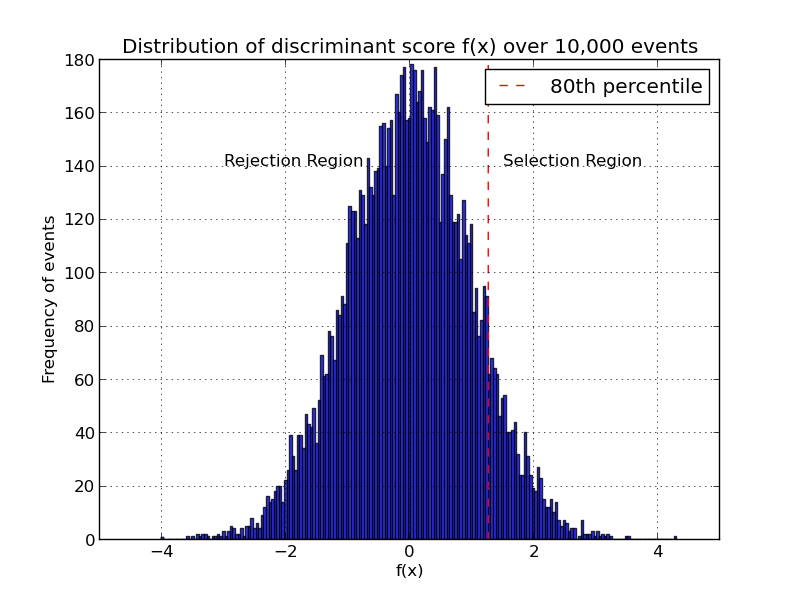
\includegraphics[scale=0.4]{Images/Selection_region.png}
\caption{This figure shows the idea of the cut-off ($\theta$) on the discriminant scores. The points to the right of $\theta$ are the predicted positives.}
\end{figure}

Below are the steps required to compute the AMS value for a classifier $h$.
\begin{enumerate}
\item Select a threshold $\theta$ for the discriminant score $f(\textbf{x})$ by choosing a percentile level $Q_{k}$.
\item Compute selected signal $s$ and background events $b$ using the importance weights provided, as in eq. \ref{unbiased}. 
\item Compute $AMS_{s}$.
\end{enumerate}

It is interesting to note the relationship between the simplified AMS metric $s/\sqrt{b}$ and the \textit{Receiver Operating Characteristic} (ROC) curve \footnote{The rather unusual name ROC emerged during World War II for the analysis of radar images. Radar operators had to decide whether a blip on the screen was an enemy target, friendly ship or just noise. Signal detection theory measures the ability of radar receiver operators to make these import distinctions. Their ability to do so was called \textit{Receiver Operating Characteristics}}.  The ROC curve illustrates the performance of a binary classifier by plotting the true positive rate (TPR = TP/P), also called \textit{sensitivity} against the false positive rate (FPR = FP/N). A fixed discriminant threshold gives a single TPR and FPR (a single point on the curve), the curve is generated by computing the TPR and FPR for different values of the discriminant threshold. Fig. \ref{roc} is an example of ROC curves for 3 different classifiers. 

\begin{figure}
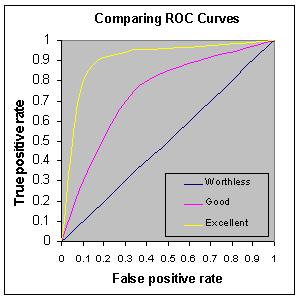
\includegraphics[scale=3]{Images/Comparing_ROC.jpg}
\caption{ROC curves for classifiers with different levels of prediction accuracy}
\label{roc}
\end{figure}

The $45^\circ$ line denotes a random classifier, which at no threshold gives a higher TPR than FPR. An ROC curve that lies above the $45^\circ$ denotes a classifier with higher than random classification accuracy of positive samples for all values of the threshold and encloses a larger area under the curve. A perfect classifier has a TPR = 1 and FPR = 0 denoting perfect accuracy. The closer the ROC curve for a classifier is to the upper left corner of the graph (1,0) the more accurate the classifier. The value on the $x$-axis, the FPR is also expressed as (1 - \textit{specificity}), where  specificity is the true negative rate (TN/N).

The slope of the tangent line to the ROC curve at a fixed threshold is the ratio $\frac{\displaystyle TPR}{\displaystyle FPR}$. This is also called the positive likelihood ratio $(LR+)$, 

\begin{equation} 
LR+ = \frac{TPR}{FPR} = \frac{sensitivity}{(1 - specificity)} 
\end{equation}

It is easy to see that this ratio (slope of the tangent line) is maximised at the extreme upper-left hand corner of the ROC curve, this is the point that gives the best trade-off between  the true positive rate and false positive rate. It is a reasonable approach in binary classification try to maximise the LR+ of a classifier in order to improve its overall classification accuracy.

Recall that the AMS metric $(s/\sqrt{b})$ is essentially the ratio of true positives to false positives in a selection region $\mathcal{H}$ specified by a cut-off threshold $\theta$. Maximizing the AMS is tantamount to maximizing the true positives and minimizing the false positives in the selection region. This is very close to the idea of maximizing the positive likelihood ratio $(LR+)$. However, there are two fundamental differences between the idea of the AMS and the ROC.

\begin{enumerate}
\item Computing the ratio of true positives to false positives in the AMS metric is tied to importance weights associated with samples in the selection region, 
\begin{displaymath}
\frac{s}{\sqrt{b}} = \frac{\sum_{i \in \mathcal{S}\cap\hat{\mathcal{H}}} w_{i}}{\sqrt{\sum_{i \in \mathcal{B}\cap\hat{\mathcal{H}}} w_{i}}}
\end{displaymath}This distorts the relationship between the likelihood ratio and AMS metric. It is possible to achieve a higher AMS metric at a point on the ROC curve where the LR+ ratio is not maximized.
\item{The area under the ROC curve, also called AUC or ROC\_AUC score integrates over all possible values of the cut-offs while the AMS considers a single point. It is computed by fixing a cut-off and ignoring all samples outside that cut-off.}
\end{enumerate}

The numerator and denominator of the LR+ ratio are rates rather than counts. The TPR = TP/P and FPR = FP/N, hence TPR/FPR = (TP/FP)*(N/P). In AMS we are dealing with counts, the actual number of true positives and false positives which are estimated as sum over importance weights. In the absence of weights the two ratios would be more homogeneous but in the presence of weights they are more de-linked. 
It is clear that optimizing the ROC curve is not the same as optimizing for the AMS. 

The \textit{precision} metric which is calculated as, $\frac{\displaystyle FP}{\displaystyle TP+ FP}$ is also closely related to the AMS metric. The precision of a classifier is (1 - False Discovery rate (FDR)) where $FDR = \frac{\displaystyle FP}{\displaystyle TP+ FP}$. In a ranked set of events (rank by value of discriminant score $f(\textbf{x})$ where the candidate signals come first), we are interested in estimating with confidence the fraction of falsely discovered events \cite{RM}. This is because highly ranked false discoveries (false positives) bring the AMS value down as they end up in the selection region. However, optimizing for precision or FDR is not an equivalent objective to the AMS as the former is a mere fraction of correct predictions and does not incorporate importance weights. 

\subsection{AMS and Balanced Classification Error}
\label{AMSbce}
A metric that closely matches the fluctuations in the AMS must incorporate the importance weights. One that is proposed by ATLAS physicists is the \textit{balanced classification error}. It is defined as, 

\begin{equation} 
R(f) = \sum_{i=1}^{n}w_{i}'\mathbb{I}\{y_{i}^{pred} \neq y_{i}^{true}\}. 
\label{bce}
\end{equation}

$\mathbb{I}$ is the indicator function. The weights $w_{i}'$ are normalized in both the signal and background classes to $N_{b}' = N_{s}' = 0.5$, that is, 

\begin{equation}
w_{i}' = w_{i}  \hspace{2mm} \times 
\begin{cases}
\dfrac{1}{2N_{s}} & \textrm{ if } i \in \mathcal{S} \\
\dfrac{1}{2N_{b}} & \textrm{ if } i \in \mathcal{B} 
\end{cases}
\end{equation}
 
A classifier is trained to minimize the balanced classification error as in eq. \ref{bce}. The AMS is then optimized with respect to a selection threshold $\theta$ in the classifier that classifies according to $sign(f(\textbf{x}) - \theta)$. Prior experiments at ATLAS suggest that the AMS is optimized at a threshold $\theta$ yielding a selection region $\mathcal{H} = \{ \textbf{x} : f(\textbf{x}) > \theta \}$ that is a small subset of the positive region $\{ \textbf{x} : f(\textbf{x}) > 0\}$ defined by the balanced classifier $sign(f(\textbf{x}))$.

It is important to re-balance the weights used in the classification error in order to penalize misclassified signals as severely as misclassified background events. Recall that the original weights $w_{i}$ for signal events are on average 300 times smaller than those for background events. %The AMS is \textbf{always} computed on unnormalized weights as in eq. \ref{weights}

\section{Support Vector Machines (SVM)}
\label{SVM}

This section lays the foundation of the SVM algorithm used on the Higgs dataset. It describes the mathematical framework of the algorithm and how it is applied to the task of binary classification. We briefly talk about why it works as a reasonable classifier on the dataset at hand. 
 
Support vector machines are an extension of the idea of \textit{maximum margin separating hyperplanes}. In a binary classification task of 2-dimensional feature vectors the maximum margin hyperplane is a linear line that divides the feature space such that the margin between the points on either side of the line closest to the boundary is maximized. The notion of \textit{margin} refers to euclidean distance.

\begin{figure}
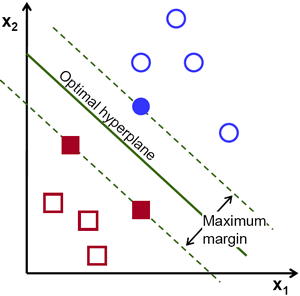
\includegraphics[scale=2]{Images/optimal_hyperplane_linear.png}
\caption{Separating hyperplane for a 2-class, 2-feature example}
\label{2line}
\end{figure}

Points on either side which lie closest to the  separating line are called \textit{support vectors}, see figure \ref{2line}. Sections \ref{primal} and \ref{dual} will prove that in a general $n$ dimensional feature space the parameters of the separating hyperplane are fully determined by the support vectors.

For a 3-dimensional feature space, the decision boundary is a 2-dimensional plane.  

\begin{figure}
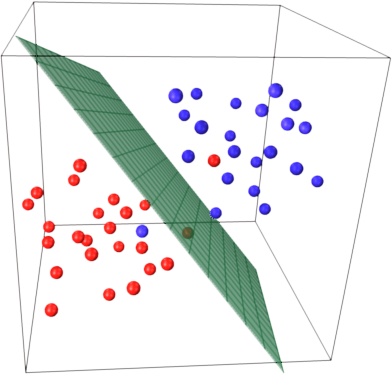
\includegraphics[scale=0.5]{Images/3D_LinearSVM.png}
\caption{Separating hyperplane for a 2-class, 3 feature example. Note : in the figure the red and blue classes are not linearly separable.}
\end{figure}

For an $n$-dimensional feature space the SVM tries to find an optimal $(n-1)$-dimensional separating hyperplane that divides the $n$-dimensional space into two parts. 

\subsection{Equation of a hyperplane}

Hyperplanes generalize the usual notion of a plane in $\mathbb{R}^3.$
A hyperplane can be expressed as a set of points satisfying, $H =\{\vec{x} : \vec{w}.\vec{x} + b = 0\}$ where $\vec{w} \in \mathbb{R}^n$ is the normal vector \footnote{The normal to the hyperplane is a vector $\perp$ to it at a point.} to the hyperplane, and $\vec{x}$ is an $n$-dimensional real vector. 

The equation of a hyperplane is defined by a point $P_{0}$ and a perpendicular vector to the plane $\vec{w}$ at that point. 

\begin{figure}
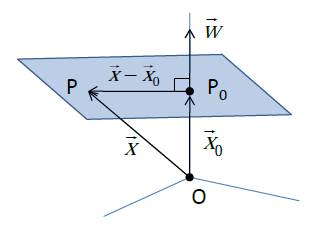
\includegraphics[scale=0.7]{Images/hyperplane.png}
\caption{Vector representation of hyperplane}
\end{figure}

Let $\vec{x_{0}} = \vec{OP_{0}}$ and $\vec{x} = \vec{OP}$, $P$ is an arbitrary point on the hyperplane. For P to be on the hyperplane, the vector $\vec{x} - \vec{x_{0}}$ must be perpendicular to $\vec{w}$. This implies, 

\begin{align}
\vec{w}.(\vec{x} - \vec{x_{0}}) = 0  \\
\vec{w}.\vec{x} - \vec{w}.\vec{x_{0}} = 0
\end{align}

Defining $b = -\vec{w}.\vec{x_{0}}$ gives, $$\vec{w}.\vec{x} + b = 0$$ This equation holds for $\mathbb{R}^n$ when $n > 3$. 

When the $b$ coefficient changes the hyperplane moves along the direction of $\vec{w}$, two hyperplanes with different $b$ coefficients are parallel to each other. Distance between parallel hyperplanes $\vec{w}.{x} + b_{1} = 0$ and  $\vec{w}.{x} + b_{2} = 0$ is $D = \dfrac{|b_{1} - b_{2}}{||\vec{w}||}$ 
$(||\bullet|| \textrm{ denotes vector length) }$

\subsection{Derivation of the Primal} 
\label{primal}

In the case of linearly separable data we can select two parallel hyperplanes that separate the two classes such that the distance between them is as large as possible. The region bounded by these two parallel planes (see figure \ref{2line}), is the \textit{margin}, and the optimal hyperplane lies in the midpoint of this region. 

We are given a training dataset of $N$ points of the form, $(\vec{x_{1}},y_{1}),...,(\vec{x_{N}},y_{N})$ where the $y_{i}$ are either 1 or -1, each indicating the class label for an $n$-dimensional data point $\vec{x_{i}}$. 

We introduced a general equation of the hyperplane as  $\vec{w}.\vec{x} + b = 0$, we need to find the $\vec{w}$ and $b$ that not only classifies the points correctly, but do so with the largest possible margin. Given an unknown data point $\vec{x}$ the hyperplane acts as a decision boundary for the class to which it is assigned to. 

The projection of the unknown $\vec{x}$ onto $w_{i}$, i.e. the dot product $\vec{w}.\vec{x}$ gives a number that is proportional to the length of the normal vector ($\vec{a}.\vec{b} = || \vec{a}||.||\vec{b}||cos\theta$). This idea promotes the decision rule,\\
%The larger the dot product $\vec{w}.\vec{x}$ the more likely

$\vec{w}.\vec{x_{i}} \geqslant c, \hspace{2mm} \textrm{ for some constant c } \Rightarrow y_{i} = +1 $ \\

or, without loss of generality, replacing $b = -c,$

\begin{align}
\vec{w}.\vec{x_{i}} + b \geqslant 0 \Rightarrow y_{i} = +1 \\
\vec{w}.\vec{x_{i}} + b \leqslant 0 \Rightarrow y_{i} = -1 
\end{align}

$\vec{w}.\vec{x_{i}} + b$ serves as the discriminant function $f(\textbf{x})$ of the classifier where classification decisions are based on the $sign(f(\vec{x_{i}}))$, $\vec{x_{i}}$ \textrm{ is just the vector representation of } $\textbf{x} \in \mathbb{R}^d$. However, we still do not have enough constraints to solve for $\vec{w}$ and $b$.

We introduce two additional constraints insisting that, the decision rule  $\vec{w}.\vec{x_{i}} + b$ for positive samples $x_{+}$ \footnote{A positive (negative) sample has a class label $y_{i}$ = $+1 (-1)$} gives a value  $\geqslant 1$ and for negative samples $x_{-}$, gives a value $\leqslant -1$. For each $i$, we insist, 

\begin{gather}
\label{df_11}
\vec{w}.\vec{x_{+}} + b \geqslant 1,\hspace{2mm} \textrm{ if } y_{i} = 1 \\
\vec{w}.\vec{x_{-}} + b \leqslant -1,\hspace{2mm} \textrm{ if } y_{i} = -1
\label{df_12}
\end{gather}

This has the effect of fixing a minimum separation margin of 2, [-1 to +1] for the parallels to the optimal hyperplane. With this condition it is easy to see that points on either side which lie closest to the optimal hyperplane will lie on the parallels to the hyperplane and satisfy the decision function with the equality. This gives the equations of the parallels to the hyperplane. 

\begin{gather}
\vec{w}.\vec{x_{+}} + b = 1,\hspace{2mm}  \\
\vec{w}.\vec{x_{-}} + b = -1,\hspace{2mm} 
\end{gather}

The points which satisfy the above conditions lie on the parallels to the hyperplane, recall that these are essentially the \textit{support vectors}. We will prove in section \ref{dual} that the parameters $\vec{w}$ and $\vec{b}$ of the optimal hyperplane are fully determined by these points.

Combining the decision rules in eq. \ref{df_11} and eq. \ref{df_12}, into one equation, we can re-write them as, 

\begin{equation}
\label{constraints}
y_{i}.(\vec{w}.\vec{x} + b) - 1 \geqslant 0, \textrm{ for all } 1 \leqslant i \leqslant n
\end{equation} 

The distance between the parallels to the optimal hyperplane, the \textit{margin} which we seek to maximize is given by,

\begin{equation}
D = \frac{|(b - 1) - (1 + b)|}{||\vec{w}||} = \frac{2}{||\vec{w}||}, \hspace{2mm} 
\end{equation}

This is an important derivation as it suggests that the margin is independent of $b$ and is only tied to the length of the normal vector. 

Maximizing the margin, amounts to maximizing  $\frac{\displaystyle 2}{||\displaystyle \vec{w}||}$, equivalently minimizing $||\vec{w}||$, or minimizing $\frac{\displaystyle 1}{\displaystyle 2}||\vec{w}||^{2}$ (1/2 is used for mathematical convenience in taking derivatives).

In summary the derived problem is, 

Minimize $\frac{\displaystyle 1}{\displaystyle 2}||\vec{w}||^{2}$ subject to $y_{i}.(\vec{w}.\vec{x} + b) \geqslant 1, \textrm{ for all } i = 1,..,N$.

This is the \textit{primal} statement of the SVM. The $\vec{w}$ and $b$ that solve this minimization determine the optimal hyperplane : $\vec{w}.\vec{x} + b = 0$. 

The primal is an example of a \textit{quadratic programming} problem where we try to minimize a quadratic function subject to linear constraints. An important geometric interpretation of the constraints is that the data points $i$ for which the constraint equality holds i.e. points which satisfy, $y_{i}.(\vec{w}.\vec{x} + b) = 1$ are precisely the support vectors. The constraint is said to be \textit{active} for the support vectors and \textit{inactive} for other data points which lie further away from the parallels on either side. 

\subsection{Derivation of the Dual}
\label{dual}
The primal statement involves optimizing an objective subject to a constraint. This can be expressed as the Lagrangian, 

\begin{equation}
\label{lagrange}
L = \frac{1}{2}||\vec{w}||^2 - \sum_{i=1}^N\alpha_{i}[y_{i}.(\vec{w}.\vec{x} + b) - 1],
\end{equation} 

where $\alpha_{i}$ are the Lagrange multipliers. 

Taking derivatives w.r.t \hspace{1mm} $\vec{w}$ and $b$, 
\begin{gather}
\partial L/\partial \vec{w} = \vec{w} - \sum_{i=1}^N\alpha_{i}y_{i}\vec{x_{i}} \nonumber\\
\label{dual1} \Rightarrow \vec{w} = \sum_{i=1}^N\alpha_{i}y_{i}\vec{x_{i}} \\
\partial L/\partial \vec{b} =  - \sum_{i}^N\alpha_{i}y_{i} \nonumber\\
\label{dual2} \Rightarrow \sum_{i=1}^N\alpha_{i}y_{i} = 0
\end{gather}

Substituting conditions \ref{dual1} and \ref{dual2} in the Lagragian \ref{lagrange}, we get, 

\begin{multline*}
L =  \frac{1}{2}\left(\sum_{i=1}^N\alpha_{i}y_{i}x_{i}\right)
\left(\sum_{j=1}^N\alpha_{j}y_{i}x_{i}\right) \hspace{2mm} - \hspace{2mm} \left(\sum_{i=1}^N\alpha_{i}y_{i}x_{i}\right)
\left(\sum_{j=1}^N\alpha_{j}y_{j}x_{j}\right) \\ 
- \sum_{i=1}^N\alpha_{i}y_{i}b + \sum_{i=1}^N\alpha_{i}
\end{multline*}
Simplifying further, 
\begin{equation}
\label{lagrange2}
L = \sum_{i=1}^N\alpha_{i} - \frac{1}{2}\sum_{i=1}^N\sum_{j=1}^N\alpha_{i}\alpha_{j}y_{i}y_{j}x_{i}x_{j}
\end{equation} subject to 
\begin{equation*}
\alpha_{i} \geqslant 0,  \textrm{ for all }  i = 1...N
\end{equation*}
\begin{equation*}
\sum_{i=1}^N\alpha_{i}y_{i} = 0
\end{equation*}

This is the \textit{dual} of the SVM problem.

The dual formulation provides some important insights into the SVM algorithm, they are summarized below :

\begin{enumerate}
\item{The dual structure of the problem highlights that the optimization problem depends on the dot product of pairs of samples (a sample is an input feature vector), $x_{i}.x_{j}$.}
\item{Moreover, the $\alpha_{i}$'s in the Lagragian in eq. \ref{lagrange} are zero for $\vec{x_{i}}$ that lie on the correct side of the hyperplane (these are the samples for which the constraints in eq \ref{constraints} are inactive) and $\alpha_{i} > 0$ for the $\vec{x_{i}}$ that lie on the parallels to the optimal hyperplane (these are the samples for which the constraints in eq. \ref{constraints} are active). This essentially reduces the dependence of the optimization problem from all data points $N$ to just the support vectors for which $\alpha_{i} > 0$.}
\item{A new data point $\vec{x_{k}}$ is classified according to the $sign(\vec{w}\vec{x_{k}} + b)$ where $\vec{w}$ is expressed as the linear combination of support vectors as derived in eq. \ref{dual1}. The offset $b$ is recovered by finding a $\vec{x_{i}}$ with an active constraint and solving, $y_{i}(\vec{w}\vec{x_{i}} + b) = 1$. The discriminant function $f(\textbf{x})$ of the classifier is,
\begin{gather}
f(\vec{x_{k}}) = \sum_{i=1}^N\alpha_{i}y_{i}x_{i}x_{k} + b, \\
\textrm{ where } \alpha_{i} \neq 0,\textrm{ only for support vectors } \nonumber
\end{gather} Hence, the decision rule depends on the dot product of support vectors with the new data point $\vec{x_{k}}$. Classification decisions are reached by looking at $sign(f(\vec{x_{k}}))$.}
\item{The fact that the entire algorithm depends on dot products between input feature vectors enables the use of \textit{kernels} in the classification problem. The idea behind using kernels for classification is the next stage of SVM algorithm, enabling it to learn in high dimensional spaces. Kernels are described in the next section.}
\end{enumerate}

\subsection{The Kernel trick : Non-linearly Separable data}
The data for classification is not always linearly separable, in this case a linear decision boundary acts as a weak classifier. Consider such a dataset in figure, \ref{nonlinear}. Clearly, there is no linear boundary that could serve as a decent classifier. 
\begin{figure}
\hspace{-9mm}
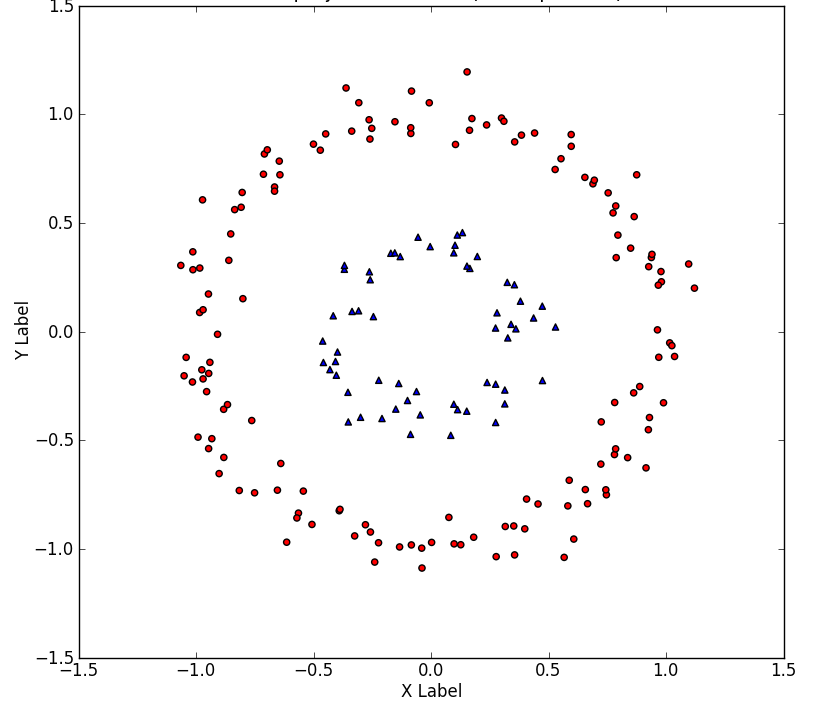
\includegraphics[scale=0.4]{Images/nonlinear_2d.png} 
\caption{Nonlinearly separable classes with 2 features}
\label{nonlinear}
\end{figure}

Suppose, we decide to map every data point in the 2 dimensional feature space ($x_{1}, x_{2}$) using a transformation (applied to the coordinates of the vector) say, $\phi : \mathbb{R}^2 \rightarrow \mathbb{R}^3$ defined as,

\begin{equation}
(x_{1},x_{2}) \rightarrow (x_{1},x_{2},x_{1}^2 + x_{2}^2)
\label{transformation}
\end{equation}

This is essentially transforming a 2-dimensional feature space to a higher dimensional one. The motive behind this transformation is that given a set of training data that is not linearly separable, one can achieve linear separability with a higher probability by projecting the data onto a higher-dimensional space via some non-linear transformation $\phi$. This is the statement of \textit{Cover's theorem} and serves as a theoretical foundation for the use of kernel methods in machine learning applications. \cite{Cover}

\begin{figure}
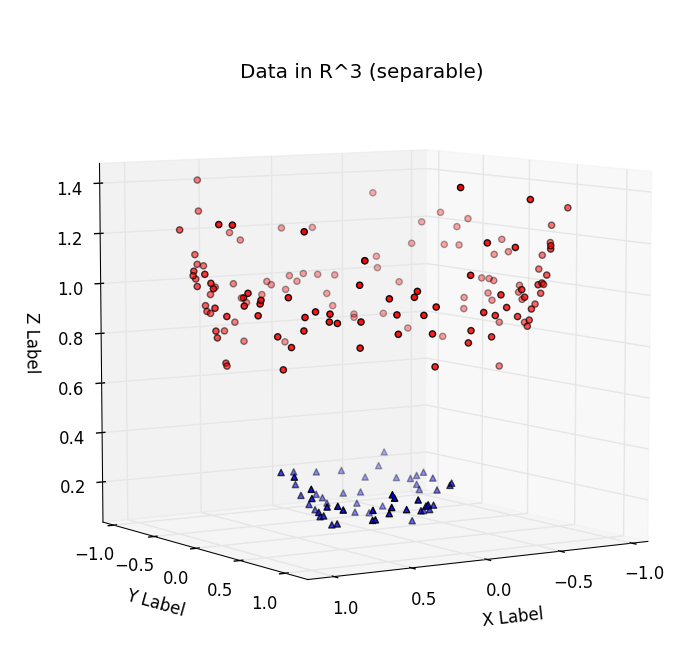
\includegraphics[scale=0.4]{Images/nonlinear_3d.png} 
\caption{Transformed feature space for data in fig. \ref{nonlinear}. The $z$ coordinate is given by $x_{1}^2 + x_{2}^2$}
\end{figure}

The features in the figure \ref{nonlinear} are now tranformed using the transformation function $\phi$ defined in eq. \ref{transformation}
Note, the non-linear transformation of the feature vector $\vec{x_{i}} \rightarrow \phi(\vec{x_{i}})$ is \textbf{not} the Kernel trick.

Assume for a moment that we have identified a transformation $\phi$ which transforms each feature vector $\vec{x_{i}} \mapsto \phi{(\vec{x_{i}})}$. The SVM training will occur on the transformed data points $(\phi{(\vec{x}_{1})}...\phi{(\vec{x}_{N})})$ and each new label $\vec{x_{k}}$ will be classified according to the sign of the discriminant function $f(\vec{x_{k}})$ where, 

\begin{equation}
f(\vec{x_{k}}) = \sum_{i=1}^N\alpha_{i}y_{i}\phi{(x_{i})}^{T}\phi{({x_{k})}} + b \footnote{When $\vec{x_{i}} \mapsto \phi{(\vec{x_{i}})}, \textrm{ then } \vec{x_{i}}.\vec{x_{j}} \mapsto \phi{(x_{i})}^{T}\phi{(x_{k})}$ }
\end{equation}

We noted earlier how the classifier depends upon dot products of pairs of input feature vectors rather than individual feature vectors. The dot product in the transformed feature space is  $\phi{(x_{i})}^{T}\phi{(x_{k})}$. The action of explicit computation of coordinates in higher dimensional space and then taking dot products can be replaced by a \textit{kernel} function $k$ which has the key property,
\begin{equation}
k(\vec{x_{i}},\vec{x_{j}}) = \phi{(x_{i})}^{T}\phi{(x_{j})} = \langle \phi{(x_{i})},\phi{(x_{j})} \rangle_{M}
\end{equation}
where  $\langle\cdot,\cdot\rangle_{M}$ is an inner product in $\mathbb{R}^M$.

Kernel functions, $\mathbf{K} : \mathbb{R}^N \times \mathbb{R}^N \rightarrow \mathbb{R}$ essentially enable computation of dot products between vectors $\vec{x_{i}}, \vec{x_{j}} \in \mathbb{R}^N$ without explicitly transforming them using $\phi$ into $\mathbb{R}^M$ where $M > N$. Further, the computation of $k(\vec{x_{i}},\vec{x_{j}})$ may be inexpensive even though $\phi{(x_{i})}$ may be expensive to calculate due to its high dimensionality. The main insight is that the SVM can be made to learn in high dimensional feature space given by $\phi$ without ever explicitly representing the vectors as $\phi(\vec{x_{i}})$. This is the \textit{kernel} trick.

To make it clear with an example, let $x, y \in \mathbb{R}^2$, consider the kernel function, 

\begin{equation}
k(x,y) = (1 + {x}^T{y})^2 \textrm{ where } x, y \in \mathbb{R}^2
\end{equation}

This can be written as, 
%\begin{align}
%\begin{split}
\begin{gather*}
k(x,y) = 1 + 2x^Ty + (x^Ty)^2 \\
\Rightarrow 1 + 2x_{1}y_{1} + 2x_{2}y_{2} + x_{1}^2y_{1}^2 + x_{2}^2y_{2}^2 + 2x_{1}x_{2}y_{1}y_{2} \\
\Rightarrow (1 + \sqrt{2}x_{1} + \sqrt{2}x_{2} + x_{1}^2 + x_{2}^2 + \sqrt{2}x_{1}x_{2}) \hspace{4mm} \times\\
\hspace{8mm} (1 + \sqrt{2}x_{1} + \sqrt{2}x_{2} + x_{1}^2 + x_{2}^2 + \sqrt{2}x_{1}x_{2}) \\
\Rightarrow \phi(x)^T\phi{y}
\end{gather*}
%\end{split}
%\end{align}
%\left( \sum_{i=1}^N\vec{x}\vec{y}\right)\left( %\sum_{j=1}^N\vec{x}\vec{y}\right) \\
%&= \sum_{i=1}^N\sum_{j=1}^N \vec{x_{i}}\vec{x_{j}}\vec{y_{i}}\vec{y_{j}}

One advantage of kernel functions is that the complexity of the optimisation remains solely dependent on the dimensionality of the input space and not of the feature space. Hence, it is possible to operate in a theoretically infinite dimensional feature space. We will see in section \ref{rbf} how the gaussian kernel corresponds to an infinite dimensional feature mapping $\phi$. 

A more intuitive representation of kernels is provided by Andrew Ng . If two vectors $\vec{x}$ and $\vec{y}$ are close together, it is reasonable to expect $k(\vec{x},\vec{y}) = \phi({x})^T\phi({y})$ to be large. Conversely, if $\phi({x})$ and $\phi({y})$ are far apart, say nearly orthogonal to each other - then $k(\vec{x},\vec{y})$  is likely to be small. So, $k(\vec{x},\vec{y})$ can be thought of as a measure of similarity between two input vectors. 

Broadly speaking, given a candidate function $k$, we can tell if it could serve as a valid kernel if $\exists$ a transformation $\phi$ such that, 

\begin{equation}
k(x,y) = \phi(x)^T\phi(y) \hspace{5mm} \forall x,y \in \mathbb{R}^N
\end{equation}

In practice, a selected group of kernels turn out to be appropriate to use in SVMs and are widely applicable to a broad class of classification problems.

\begin{table}[ht]
\caption{Popular kernel choices for SVM classification}
%\resizebox{400pt}{!}{
\begin{tabular}{p{2cm}p{3cm}p{2cm}}
\toprule
Type & Function & Parameters \\
\midrule
\rule[-2ex]{0pt}{2.5ex} Polynomial & $k(x,y) = (x^Ty + \theta)^d$ & $d$ $\theta$ \\
\pbox{10cm} {Gaussian \\(Radial Basis \\ Function)} &  $k(x,y) = e^{\lbrace\frac{-1}{2\sigma^2}||x-y||^2\rbrace}$ & $\gamma = \frac{-1}{2\sigma^2}$ \\ \\
\rule[-2ex]{0pt}{2.5ex} \pbox{20cm}{Sigmoid \\Kernel} & $k(x,y) = tanh(\eta xy + \theta)$ & $\eta$ and $\theta$ \\
\pbox{20cm} {Spectrum \\Kernel\\ for strings} & \pbox{20cm}{Count the number of \\ sub-strings in common} & \pbox{20cm}{It is a kernel since \\it is a dot product \\between vectors of \\indicators of \\substrings.} \\
\bottomrule
\end{tabular}
\label{kernels}
\end{table} 

It is worthwhile mentioning that there is no best choice in choosing a kernel for a SVM classification problem. The best approach is to try various kernels, adjust their parameters via search and minimize the generalization error.
  
The discussion surrounding what properties a valid kernel function needs to satisfy is beyond the scope of this study.  

\subsection{Kernel SVM}

To summarize, the reformulation of the dual under a kernel functions is,

\begin{equation}
L = \sum_{i=1}^N\alpha_{i} - \frac{1}{2}\sum_{i=1}^N\sum_{j=1}^N\alpha_{i}\alpha_{j}y_{i}y_{j}k(\vec{x_{i}}\vec{x_{j}})
\label{kernel_lagrange}
\end{equation}
\begin{equation*}
\alpha_{i} \geqslant 0,  
\end{equation*}
\begin{equation*}
\sum_{i=1}^N\alpha_{i}y_{i} = 0 \textrm{ for all }  i = 1...N
\end{equation*}
The parameter $\vec{w}$ of the optimal separating hyperplane, expressed under the non-linear transformation $\phi$ is, 

\begin{equation*}
\vec{w} = \sum_{i=1}^N\alpha_{i}y_{i}\vec{x_{i}}
\end{equation*}

The discriminant function $f(\textbf{x}), \hspace{1mm} \textbf{x} \in \mathbb{R}^d$ (with a vector representation $\vec{x}$) of the classifier is given by the equation of the hyperplane, 

\begin{equation*}
\vec{w}.\vec{x} + b = \sum_{i=1}^N \alpha_{i}y_{i}k(\vec{x_{i}}\vec{x}) + b = 0
\end{equation*}
where $\alpha_{i}$'s are the optimal lagrange multipliers obtained by minimizing eq. \ref{kernel_lagrange} above and offset $b$ is found by solving,
$b = 1 - \vec{w}\vec{x_{i}}$ for a support vector $\vec{x_{i}}$.

The classification decision for a new data point $\vec{x_{k}}$ is reached by looking at,

\begin{equation}
sign(f(x_{k})) = sign\left(\sum_{i=1}^N \alpha_{i}y_{i}k(\vec{x_{i}}\vec{x}) + b  \right)
\label{kernel_classify}
\end{equation}

Recall, that $\alpha_{i}$'s are 0 for data points $\vec{x_{i}}$ which lie away from the margin, the remaining data points are the support vectors. Hence, the classification decision is entirely dependent on the dot product of support vectors under a kernel function.  

The $alpha_{i}$s which $> 0$ are called the dual coefficients and temper the role played by each support vector in the classification decision. 

\subsection{Gaussian (RBF) Kernel}
\label{rbf}

The gaussian kernel, uses a radial basis function whose value depends on the notion of euclidean distance from a point. It is defined as,  

\begin{gather}
k(x,y) = e^{\Big( \dfrac{-||x-y||^2}{2\sigma^2}\Big)}
\end{gather}
for two vectors $x,y \in \mathbb{R}^d$, $||x-y||^{2}$ is the squared euclidean distance between the two vectors. A simpler definition replacing $\dfrac{1}{2\sigma^2}$ by $\gamma$ is given by,

\begin{gather}
k(x,y) = e^{\textstyle \Big({-\gamma||x-y||^2}\Big)}
\label{gamma}
\end{gather}

This is a reasonable measure of similarity as when $x$ and $y$ are close, or $||x-y||$ is close to 0 $\Rightarrow k(x,y)$ is close to 1. Conversely, when $x$ and $y$ are far apart, $\Rightarrow k(x,y)$ is close to 0. The value of the RBF kernel conveniently ranges between zero and one.  

By using Taylor's expansion $e^{x} = 1 + x + ... + \frac{1}{k!}a^{k}$ one can see how $e^{xy}$ is a kernel with an infinite set of features corresponding to polynomial terms, hence its transformation function $\phi$ maps the original feature space to an infinite dimensional one. The kernel $k(x,y)$ gives a closed form expression for computing the dot product in this higher dimensional space even when there isn't a way to represent the vector directly in this space. The main idea is that even if a vector has infinite dimensions , similarity (expressed as a dot product) between two vectors in this space has a well-defined value. The kernel expresses the dot product through an equation that indicates what the similarity value converges to.  

A gaussian kernel applied to a support vector is an exponentially decaying function in the input feature space. Its maximum value is achieved at the support vector and it decays uniformly in all directions around the support vector leading to hyper-spherical contours of the kernel function. The SVM classifier is just a weighted linear combination of the kernel function computed between a data point and each of the support vectors. 

The idea of a gaussian kernel can be visualized for a 2-dimensional feature space, where the higher dimensional space is a hyper-surface of bumps and cavities. Bumps are created for the positive signal class as the value of the kernel functions is multiplied by $y_{i} = 1$ the class label (which is always available in supervised learning) and cavities are created for the negative class as the kernel value is multiplied by $y_{i} = -1$  peaking at the support vectors for each class. A 3d depiction of this is in fig. \ref{contour}.

%\begin{figure}[ht]
%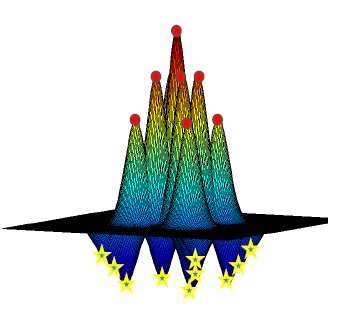
\includegraphics[scale=0.5]{Images/bumps_cav.jpg}
%\caption{RBF Kernel for 2 separable classes in 3d. Note: In this contrived example perfect separation is achieved under the RBF Kernel, however this is not always the case.}
%\label{bumps}
%\end{figure}

\begin{figure}
\hspace{-1cm}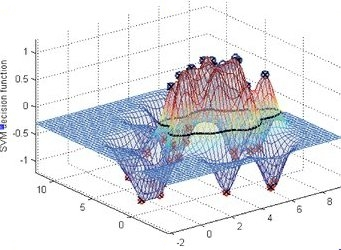
\includegraphics[scale=0.7]{Images/contour_rbf1.jpg}
\caption{RBF Kernel contour in 3d showing the bumps and cavities created by the decision values. \textit{Retrieved from \cite{RBF2}}}
\label{contour}
\end{figure}

\begin{figure}
\hspace{-1cm}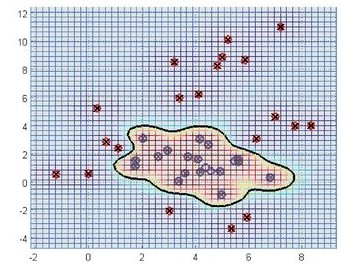
\includegraphics[scale=0.7]{Images/contour_2d_decision.jpg}
\caption{The decision boundary of the contour in figure \ref{contour} projected onto 2d. \textit{Retrieved from \cite{RBF2}}}
\end{figure}

The parameter $\gamma$ controls the width of the kernel which determines smoothness. In n-dimensions this parameter can be thought of as controlling the hyper-sphere of influence of a support vector. Again, the influence of gamma is easier to visualize in 3d. A small gamma implies larger variance (as per eq. \ref{gamma}), this leads to relatively flat peaks around support vectors, giving smoother decision boundaries and requiring few support vectors with large spheres of influence in terms of classification of other points. 

A large gamma implies lower variance and in 3d this gives a surface of sharp peaks localizing the influence of support vectors. The graphs in fig. \ref{rbf_kernels} depict the influence of three values of gamma, $\gamma = 5,10$ 

\begin{figure}
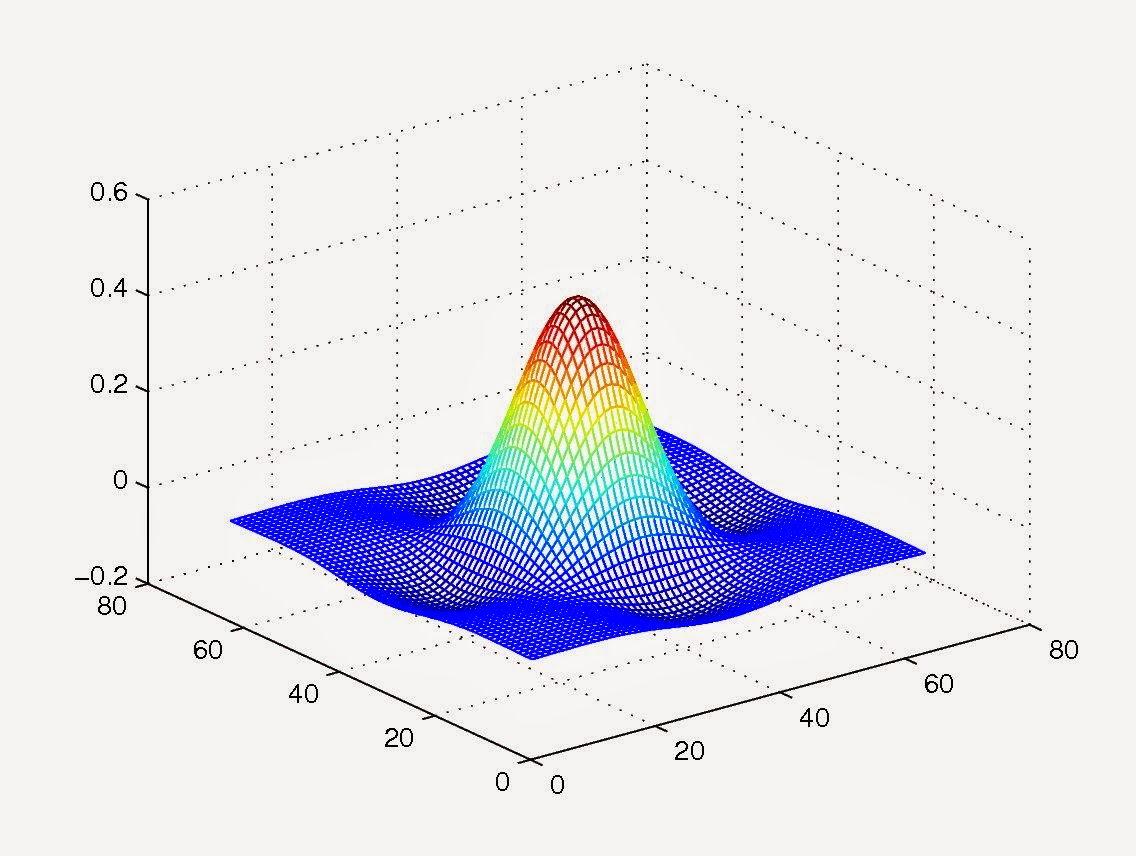
\includegraphics[scale=0.2]{Images/gamma_5.jpg}
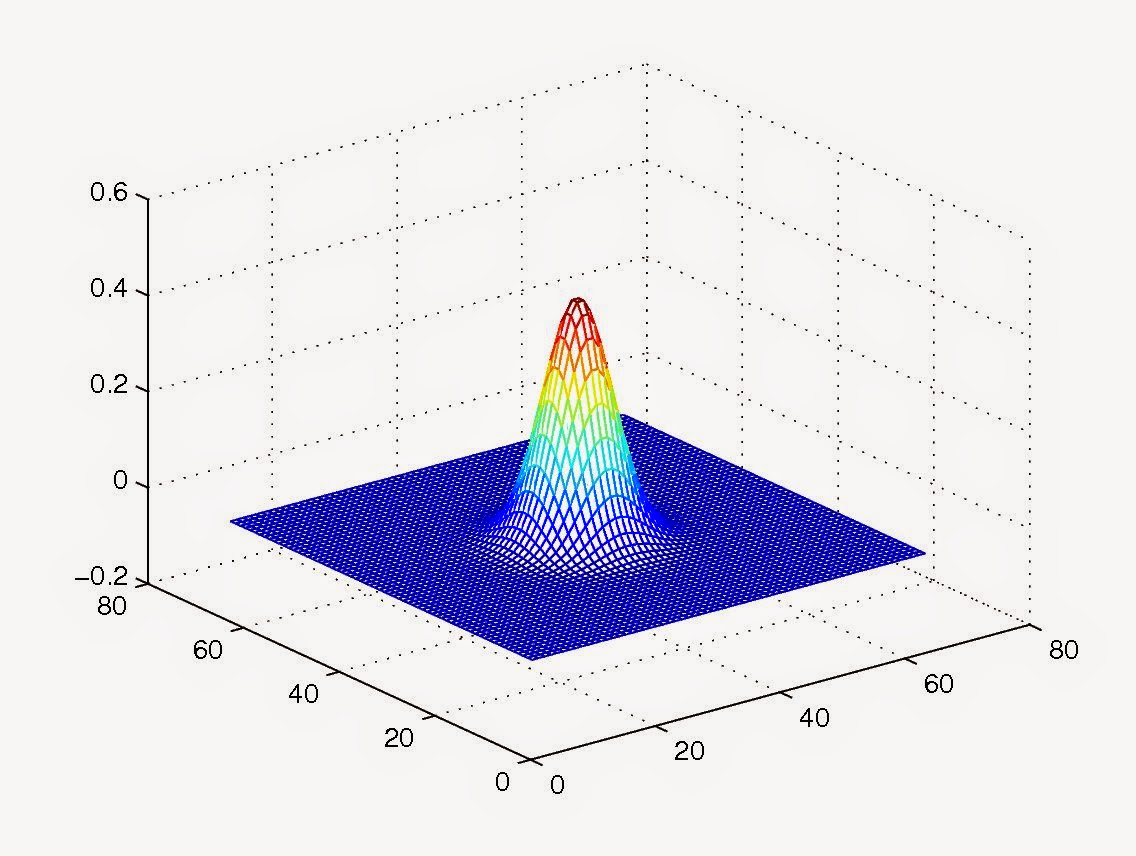
\includegraphics[scale=0.2]{Images/gamma_10.jpg}
\caption{These graphs depict the shape of a RBF kernel around a single support vector in 3d space. The top figure depicts a kernel with $\gamma$ value of 5 (flatter peak, high variance) and the bottom figure depicts a $\gamma$ value of 10 (sharper peak, lower variance). \textit{Retrieved from \cite{RBF}}}
\label{rbf_kernels}
\end{figure}

The kernels localization properties make it a strong choice of kernel for problems which need an arbitrarily flexible decision boundary. For large $\gamma$ (low variance) values, the decision boundary projected onto 2d would appear as small amorphous patches around the support vectors separating one class from the other. The depiction of this concept in 2d makes it appear like a k-nearest neighbour classifier, 

Gaussian kernels are universal kernels and give reasonable classifiers for a wide variety of classification problems. We use SVMs with gaussian kernels for the signal/background classification task in the Higgs dataset. The localization strength of a RBF kernel also explains why this is a good choice of kernel in the Higgs dataset where the classes are largely overlapping. 

\subsection{Soft Margin SVM}
\label{softsvm}

The kernel trick allows the SVM to learn by projecting non-linearly separable data to higher dimensional spaces using transformations and looking for linear boundaries. By increasing the complexity of these boundaries one can achieve perfect classification on the training data but with no real predictive power on the new data. Kernel SVMs are prone to overfitting unless carefully controlled for it. 

SVMs can be equipped with an additional parameter that controls for complexity. To introduce this parameter it is best to revisit the primal formulation of the SVM in Section \ref{primal}. In the simplest case with 2 features and 2 classes where the data cannot be perfectly separated by a optimal line, one may allow for deviations defined by $\xi_{i} > 0$ for each individual data point. The points for which $\xi_{i} = 0$ are on the right side of the boundary given by the optimal separating line, those with $\xi_{i} > 1$ are on the incorrect side of the decision boundary. Typically, $\xi_{i}$'s denote the vertical distance between the data point $\vec{x_{i}}$ and the decision boundary for points on the wrong side. This is illustrated in fig. \ref{soft_margin}

\begin{figure}
\hspace{0.5cm} 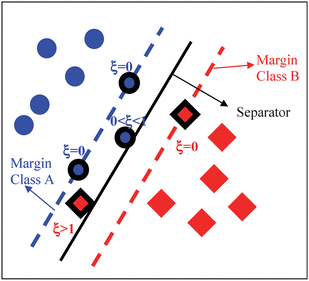
\includegraphics[scale=0.5]{Images/soft_margin.png}
\caption{Illustrating the idea behind slack variables $\xi_{i}$}
\label{soft_margin}
\end{figure}

The points that lie in the margins on either side but on the correct side of the boundary have a slack value $0 < \xi_{i} < 1$. We can see easily in this example how a linear boundary acts as a viable classifier as long as we allow some samples to be misclassified. 

All points which lie between the margins are support vectors and influence classification decisions. Intuitively, if the margins are wider, more samples fall in the enclosing region and each of them is a support vector. Less linearly separable data separated through a linear line requires wide margins so more points can be allowed to lie on the wrong side of the boundary. 

In order to build a model with slack variables for each data point, the SVM objective is modified to include a penalty term that increases in proportion to the sum of misclassification distances measured as, $\sum_{i=1}^N \xi_{i}$. The penalty term  increases linearly with $\xi_{i}$. The modified soft margin SVM primal is now written as, 

Minimize $\frac{\displaystyle 1}{\displaystyle 2}||\vec{w}||^{2} + C\sum_{i=1}^N \xi_{i}$  subject to,
\begin{align*}
\begin{split}
y_{i}.(\vec{w}.\vec{x} + b) &\geqslant 1 - \xi_{i} \\
\xi_{i} &\geqslant 0 \\
C &\geqslant 0 
\end{split}
\end{align*}
for all  i = 1,..,$N$.

The dual is expressed as, 

\begin{equation}
\label{lagrange_soft}
L = \frac{1}{2}||\vec{w}||^2 + C\sum_{i=1}^N \xi_{i} - \sum_{i=1}^N\alpha_{i}[y_{i}.(\vec{w}.\vec{x} + b) - 1 + \xi_{i}] - \sum_{i=1}^{N}r_{i}\xi_{i} 
\end{equation} 

Differentiation w.r.t $\vec{w}$ and $b$ are identical to eq. \ref{dual1} and \ref{dual2}, but now we also need to differentiate w.r.t \hspace{2mm} $\xi_{i}$, 

\begin{align}
\partial L/ \partial \xi_{i} & = C - \alpha_{i} - r_{i} \nonumber \\ 
\Rightarrow \alpha_{i} & = C - r_{i} 
\label{slack}
\end{align}

Using eq. \ref{dual1}, \ref{dual2} and \ref{slack} to eliminate $\vec{w}$, $b$ and $\xi_{i}$ we get the identical lagrangian as in the hard margin case, only with one modified constraint which arises because $r_{i} \geqslant 0 \hspace{2mm} \forall i=1,...N$.

\begin{equation}
L = \sum_{i=1}^N\alpha_{i} - \frac{1}{2}\sum_{i=1}^N\sum_{j=1}^N\alpha_{i}\alpha_{j}y_{i}y_{j}k(\vec{x_{i}}\vec{x_{j}})
\end{equation}
\begin{equation*}
0 \leqslant \alpha_{i} \leqslant C, 
\end{equation*}
\begin{equation*}
\sum_{i=1}^N\alpha_{i}y_{i} = 0 \textrm{ for all }  i = 1...N
\end{equation*}

\begin{figure*}
%\hspace{0.5cm}
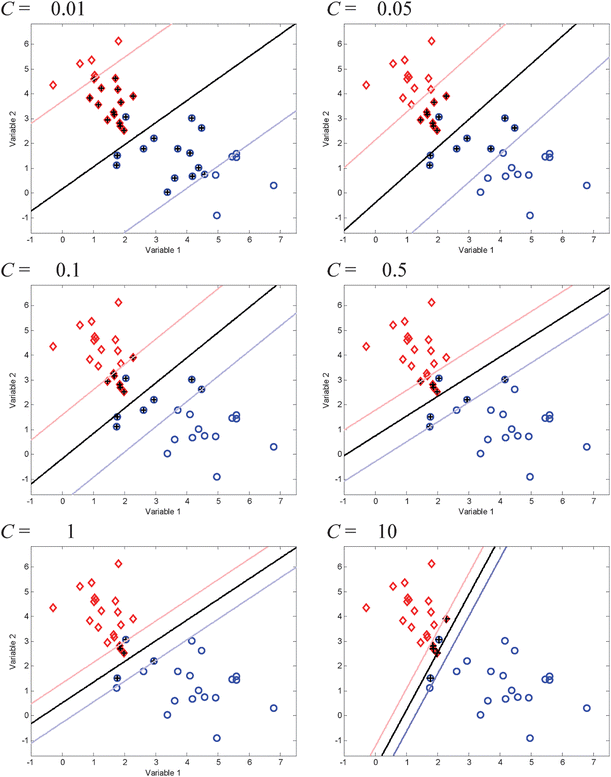
\includegraphics[scale=0.7]{Images/Changing_C.png} 
\caption{Effects of changing C on linear models. \textit{Retrieved from \cite{RBF2}}}
\label{changing_C}
\end{figure*}

Classification decisions are reached in the same way as in kernel SVMs, eq. \ref{kernel_classify}. 

The free parameter $C$ controls the trade-off between slack variable penalty and the width of the margin or in other words, model complexity (accuracy) and smoothness of the decision surface. A high C aims at penalizing misclassified points more and aims to classify all training sample points correctly, this leads to a model with a narrow margin. In the presence of kernel this would imply a highly complex decision surface. 
A low C gives a wider margin with a smaller penalty on misclassification in the training set. This also implies a smoother decision surface with a lower number of support vectors each of which with a wider sphere of influence. In hard margin SVMs $C \rightarrow \infty$ and the SVM tries to achieve perfect classification of the training set. Intuitively, $C$ is a measure of tolerance towards misclassification in a model and is an important parameter to be optimized to obtain models which strike a balance between classification error and complexity. The fig. \ref{changing_C} illustrates the effect of changing C on a linear boundary.  
 

\section{Results}

In this section we primarily discuss the results obtained by applying a soft margin SVM with a RBF kernel on the Higgs dataset. We discuss the optimization process and report the results of the model performance assessed mainly by the AMS metric. We also show performance of the model under other metrics. 
  
\subsection{The Model : Soft Margin SVM with Gaussian kernel}

For the Higgs dataset we apply a soft margin SVM with a Gaussian kernel for the binary classification task. The choice of model is justified due to the following reasons:

\begin{enumerate}
\item{We are dealing with a high dimensional dataset of 30 features with heavily overlapping class distributions, a gaussian kernel is a good universal kernel choice which allows for flexible decision boundaries.}
\item{The Gaussian kernel through the $\gamma$ parameter allows the user to control and optimize the influence of support vectors.}
\item{From the discussion in section \ref{ams} it is evident that we are not trying to achieve a perfect classifier with 100$\%$ training accuracy but a classifier that generalizes well to test data and is robust to over-fitting. Hard margin classifiers are a poor choice given that the optimization objective is not tied to accuracy.}
\item{The role of the C parameter in the soft margin SVM model is complementary to the $\gamma$ parameter, lower gamma (smooth models) can be made more complex by selecting a larger C (penalizing misclassifications) and higher gamma (complex and localized) models can be stabilized by selecting lower C (allowing misclassifications).}
\item{Since the performance of soft margin SVMs rely on the optimization of 2 parameters C and $\gamma$ on the training data set, the graphical visualization can provide intuition about the complementary nature of the parameters.}
\end{enumerate} 

Complementary nature of $C$ and $\gamma$ depicted on a small dataset of two coalesced classes. 

\begin{figure}
\hspace{-0.7cm}
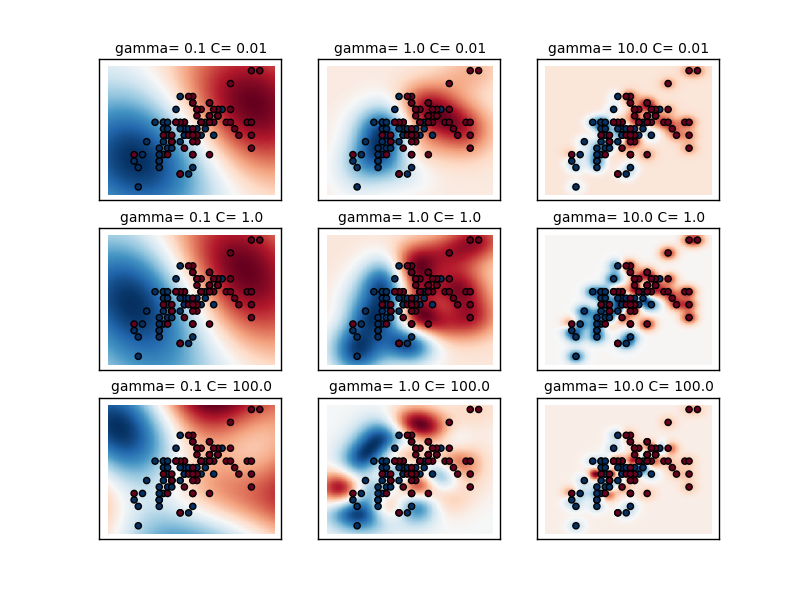
\includegraphics[scale=0.5]{Images/RBF_Params.png} 
\caption{Effects of changing C and gamma (RBF Kernel) on a 2-class overlapping dataset. \textit{Retrieved from \cite{PyRBF}}}
\label{c_gamma}
\end{figure}


\label{learning_pipe}
\subsection{Pruning of the training set}

We have explained in section 4.4 how the classification decision of an SVM classifier are solely tied to the support vectors. The support vectors are selected during the training stage of the algorithm. The selection process of support vectors  is one of the most computationally expensive parts of the SVM learning process. The training complexity of a non-linear SVM is typically $O(n^{3})$ in the number of training data points. The time complexity of running of an SVM on a new dataset is linear in the number of support vectors.

Further, the predictive power of an SVM relies entirely on the support vectors. Hence, an SVM algorithm that is trained solely on the support vectors  should be as accurate as one that is trained on the entire dataset. 

The question now is, how can we preselect samples from a population which have a high likelihood of being support vectors ?. In the two feature binary class problem, one can get a good sense of the decision boundary through visualizing the dataset. By selecting samples which lie around the decision boundary and rejecting samples which are away from the intersecting class clusters.

In higher dimensions it is hard to visualize the decision boundary and get a good sense of samples which lie on the intersection of class clusters. A surrogate idea is to select samples that cluster around the mean feature value for each of the $n$ features. We call this idea \textit{choice} sampling. 

\begin{algorithm}
\caption{Choice Sampling}
\begin{algorithmic}[1]
\FORALL{$n$ features} 
\STATE \textbf{Compute} $\mu_{i}, \sigma_{i} \leftarrow$ mean, std. deviation of the $i$-th feature. 
\STATE \textbf{Select} a factor $r$ 
\STATE \textbf{Choose} all samples $S_{i}$ that lie in $(\mu_{i}-r\sigma_{i},\mu_{i}+r\sigma_{i})$ 
\ENDFOR
\STATE $S = \bigcap S_{i} \forall i=1...n$  
\RETURN $S$
\end{algorithmic}
\label{choicealgo}
\end{algorithm}

A choice sample $S$ was constructed in this manner with $r$ = 1.6.

The entire dataset has 250,000 rows many of which have missing values. In this analysis we focus on rows which have no missing values in any of the features and as a first step condense the training set by dropping rows with any missing values. The final size of the condensed dataset with no missing values was 68114.

At this stage we have a pure sample of 68114 rows and no missing values, we then split this pure dataset into a training set (TRAIN) and test set (TEST) by uniform random selection with each data point equally likely to fall into either the TRAIN or TEST set. The respective proportions of the training and test set are 80$\%$ and 20$\%$. The TEST set is held-out only to be used for the final testing stage. 

The TRAIN set at this stage has 54491 samples (80$\%$ of the pure sample). The remaining 13623 rows are held out for testing. The choice sampling algorithm \ref{choicealgo} is run on the TRAIN set to condense the TRAIN set further. A factor $r$ of 1.6 is used to control the number of standard deviations away from the mean we want each feature value to lie in the sample. 

The size of the condensed dataset after sampling was 11,600, we call this pure sample set TRAIN$\_$CHOICE. A uniform sample of the same size was chosen on the pure dataset to compare at a later stage, the differences between the performance of the SVM classifiers fitted to them. 

\subsection{Feature Selection}

\begin{figure*}
\hspace{-2cm}
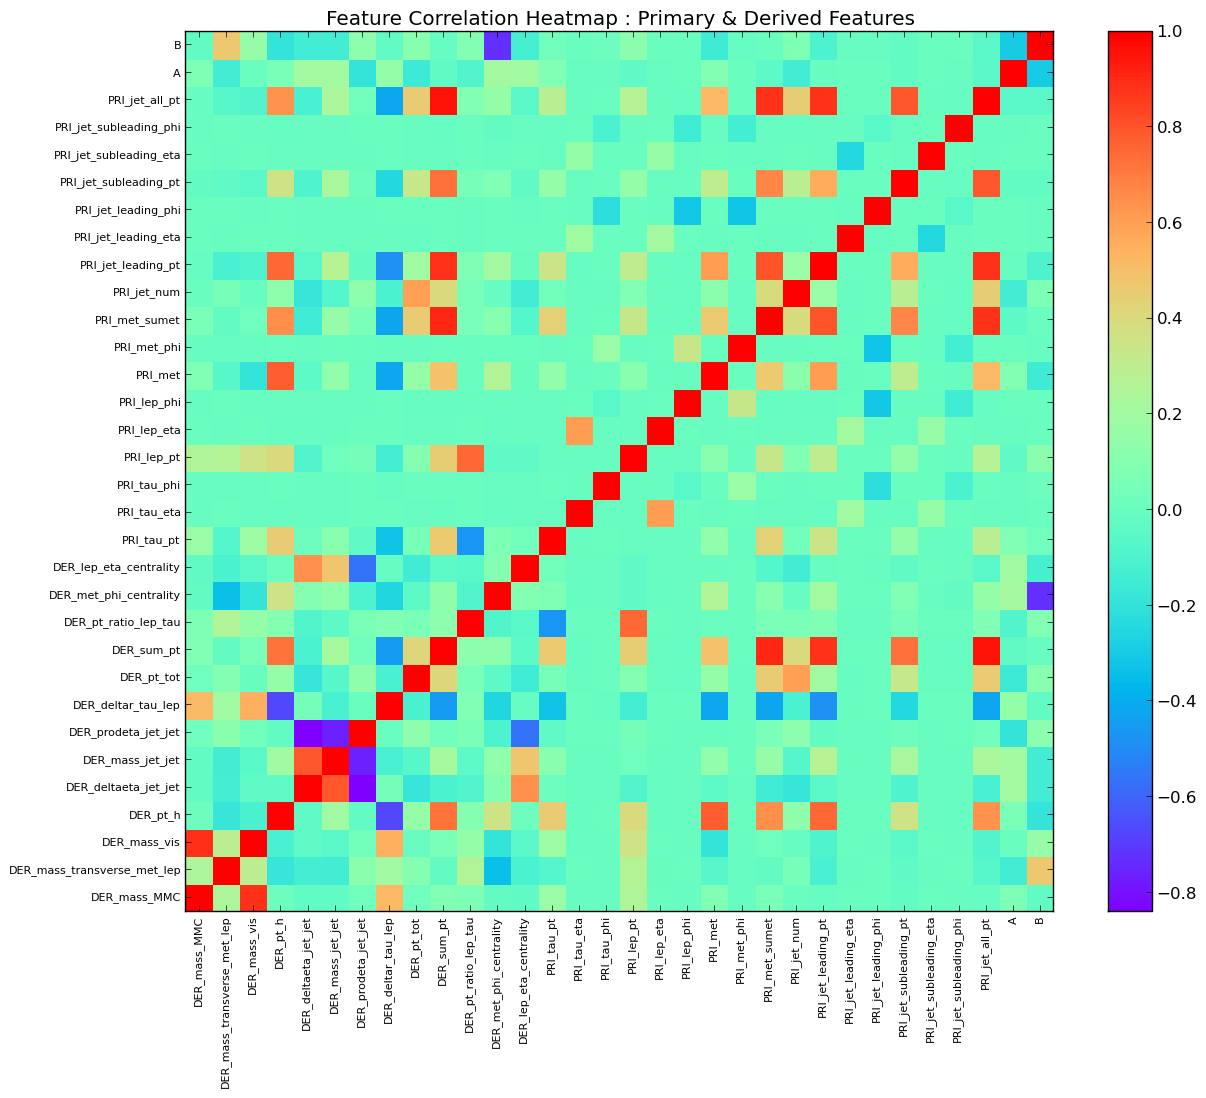
\includegraphics[scale=0.6]{Images/DERFeaturesHeatMap.png}
\caption{Feature Correlation map showing the strength of correlation between different features. It is a symmetric display with 1s on the diagonal showing correlation of a feature with itself. The features that had correlation coefficient values $|c| > 0.8$ with other features were dropped. From a group of correlated features only the one with the highest point bi-serial correlation was retained.}
\label{ff}
\end{figure*}

The feature correlation map is depicted in fig. \ref{ff}, it shows the strength of correlation between features across both classes. 

Features that are strongly correlated with other features represent low discriminating power and can be removed without much information loss. Redundant features were identified on the basis of the strength of their correlation with other features and dropped from the dataset. 

Since the class variable is dichotomous, $y_{i} \in \{0,1\} \forall i$, the feature vs. class correlation is computed using the point-biserial correlation. This is mathematically equivalent to the Pearson correlation for computing correlations between one continuous and one dichotomous variable. The point-biserial correlation was computed between each feature and the binary class variable. It is computed as, 

\begin{equation}
r_{pb} = \dfrac{M_{1} - M_{0}}{s_{n}}\sqrt{\dfrac{n_{1}n_{0}}{n^2}}
\end{equation}

where $M_{0}$ and $M_{1}$ are the mean values of the feature for the background and signal class. $s_{n}$ is the inter-class standard deviation of the feature, $n_{0}$ and $n_{1}$ represent the count of samples in the background and signal class and $n$ is the overall count. From figure \ref{biserial} it is apparent that the derived features showed higher correlation with the class label than the primary features \ref{features}. 
 
\begin{figure*}
\hspace{1.8cm}
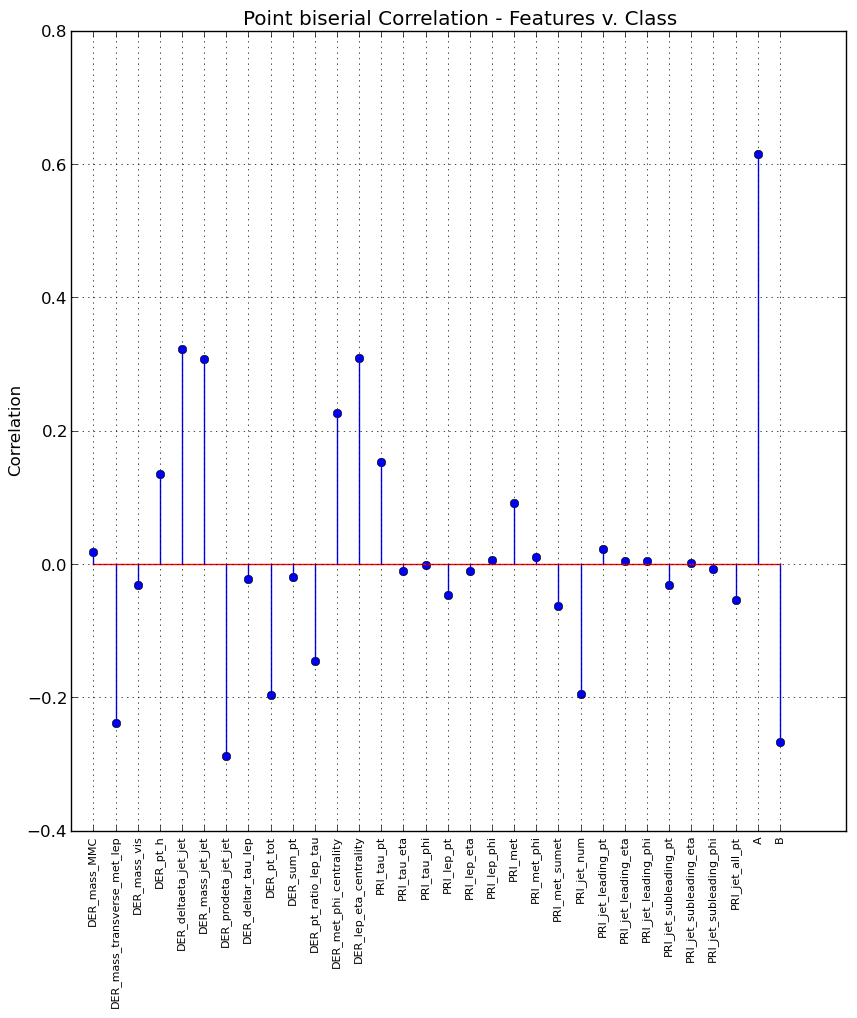
\includegraphics[scale=0.6]{Images/BiSerialCorr.png}
\caption{The figure shows the strength of correlation of derived features (DER\_$*$) over the primary features (PRI\_$*$). Derived jet features showed higher correlation and analytically derived feature A and B showed higher correlation to any of the primary features.}
\label{biserial}
\end{figure*}


\subsection{Hyper-parameter Tuning}

For an initial search I use a logarithmic base 10 grid with C ranging from $10^-2$ to $10^3 $ and $\gamma$ ranging from $10^-4$ to $10^0$. The graphs below show the effect of varying C and $\gamma$ in these ranges on two carefully chosen metrics : 

\begin{enumerate}
\item{ROC\_AUC score : This is the area under the ROC curve, although we have delved into why optimizing the ROC$\_$AUC is not equivalent to maximizing the AMS, it is a good measure of overall classification accuracy combining sensitivity and specificity. We use this metric to identify a broad region of interest.}
\item{Balanced classification error : This motivation behind this metric was discussed in section \ref{AMSbce}, it provides a way to incorporate the importance weights on each sample in a measure of accuracy.}
\end{enumerate}

The base10 grids in fig. \ref{metrics_grid10} help in identifying a trend which reaffirms the complementary relationship between $C$ and $\gamma$ discussed in section \ref{softsvm}. Viable classifiers lie on the diagonal of $C$ and $\gamma$ values, with the best parameters (C,$\gamma$) turning out to be (10,0.01), (1000,0.001). In the balanced classification error heat map we observe a similar trend of the stronger classifiers falling on the diagonal where C ranges from 10 to 1000 and $\gamma$ ranges from  0.001 to 0.01. 

\begin{figure*}
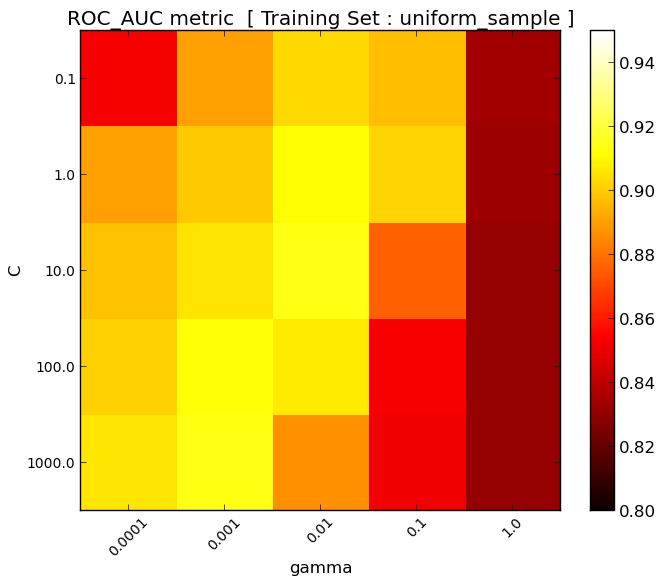
\includegraphics[scale=0.51]{Images/ROC_AUC_uniform_sample_grid10.png} 
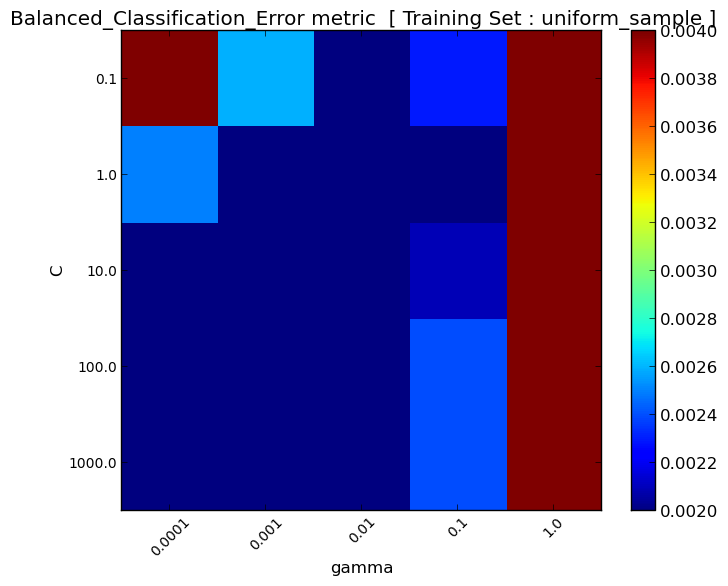
\includegraphics[scale=0.51]{Images/Balanced_Classification_Error_uniform_sample_grid10.png} 
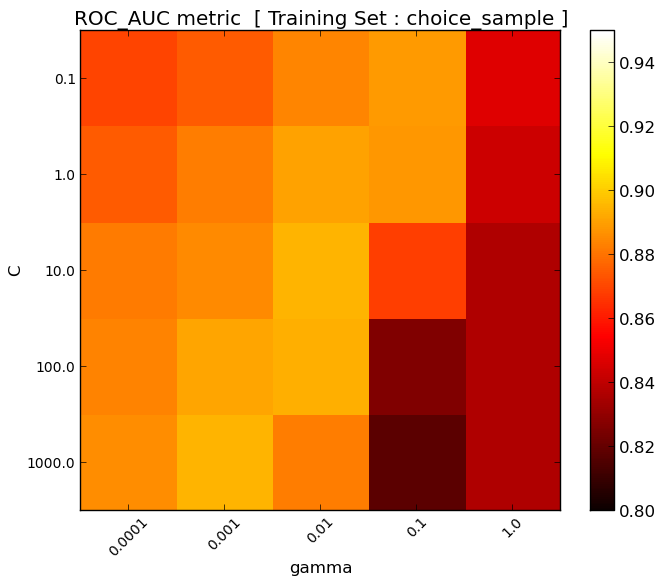
\includegraphics[scale=0.51]{Images/ROC_AUC_choice_sample_grid10.png} 
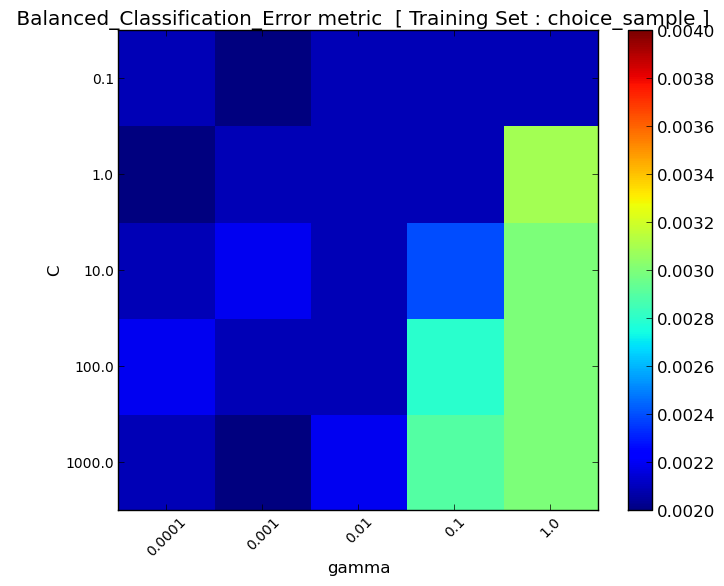
\includegraphics[scale=0.51]{Images/Balanced_Classification_Error_choice_sample_grid10.png} 
\caption{Grid search over base 10 grid of $C$ and $\gamma$ values. The uniform sample and the choice sample give very similar ROC and Balanced classification error patterns for values of $C$ and $\gamma$.}
\label{metrics_grid10}
\end{figure*}

At first glance it looks as though optimal parameters could be found if the grid were to be expanded on the bottom-left (higher C and lower $\gamma$). Indeed, good classifiers would continue to be found for higher values of C and proportionately lower $\gamma$ values. This is the bias-variance trade off in play in  SVM learning. A model with higher misclassification penalty $C$ and a smooth decision surface (low $\gamma$) can achieve the same predictive power of a model with a lower $C$ but highly complex decision surface (high $\gamma$ implies narrow localized spheres of influence around the support vectors). However, models with higher $C$ and lower $\gamma$ are computationally  more expensive that lower C and higher $\gamma$, this is because with a higher misclassification penalty and smoother decision surface, the SVM is forced to choose a large number of support vectors to maintain a decent level of accuracy. A large number of support vectors implies that a model is slow to predict. Hence, we can always bound the value of $C$ to a to favour faster and simpler models and fine tune the $\gamma$ parameter. This is something we try and achieve in the next step.

In order to demonstrate that we get equally predictive classifiers as we go down the diagonal of higher C and lower $\gamma$ we expand the score heat map to add two more additional rows with C = 10000. The plot in fig. \ref{rochigh} was constructed at the expense of a relatively higher compute time of $60$ minutes. 

\begin{figure}
%\hspace{1cm}
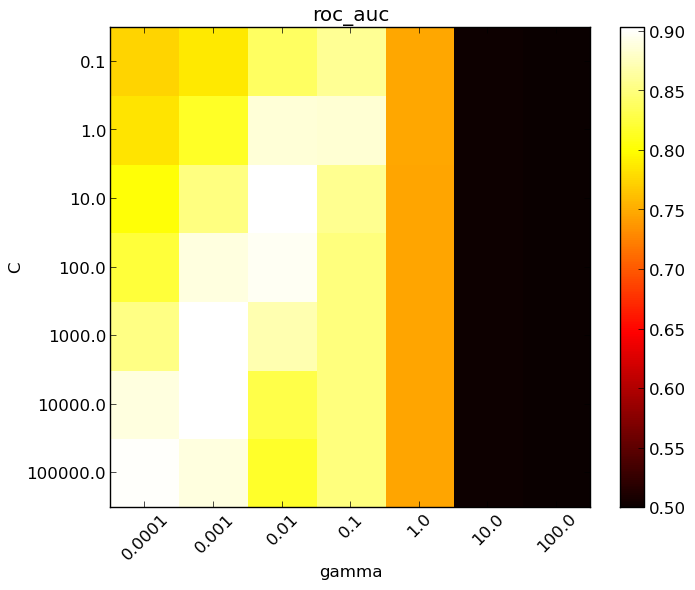
\includegraphics[scale=0.5]{Images/ROC_AUC_high.png}
\caption{Demonstrating that optimal classifiers can always be found on the diagonal of $C$ and $\gamma$}
\label{rochigh}
\end{figure}

One could argue that a choice sample is a biased sample, it is a biased sample however given the mathematical framework of SVM algorithms in which the final decision function is independent of points which are not support vectors. 

In the next step we construct a finer grid with a base2 step size to narrow down further on the optimal $\gamma$ parameter for a value of $C$ that does not exceed 1000.  

\begin{figure*}
\hspace*{-0.5cm}
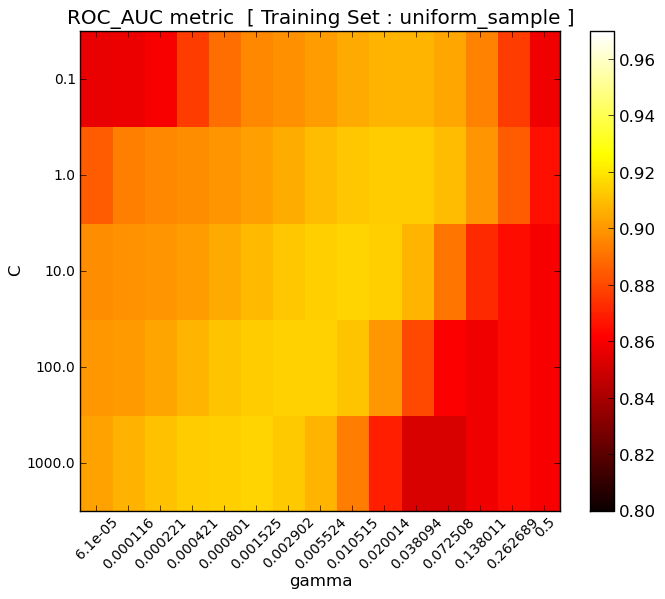
\includegraphics[scale=0.5]{Images/ROC_AUC_uniform_sample_grid2.png} 
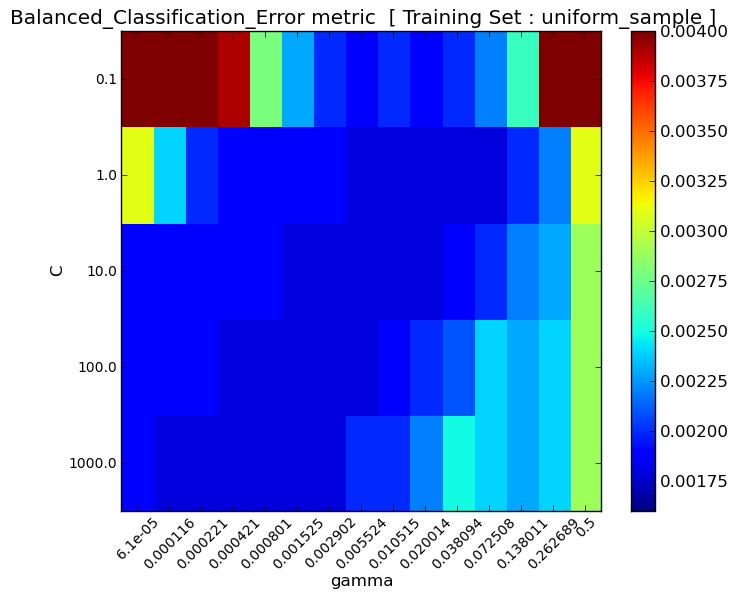
\includegraphics[scale=0.5]{Images/Balanced_Classification_Error_uniform_sample_grid2.png} 
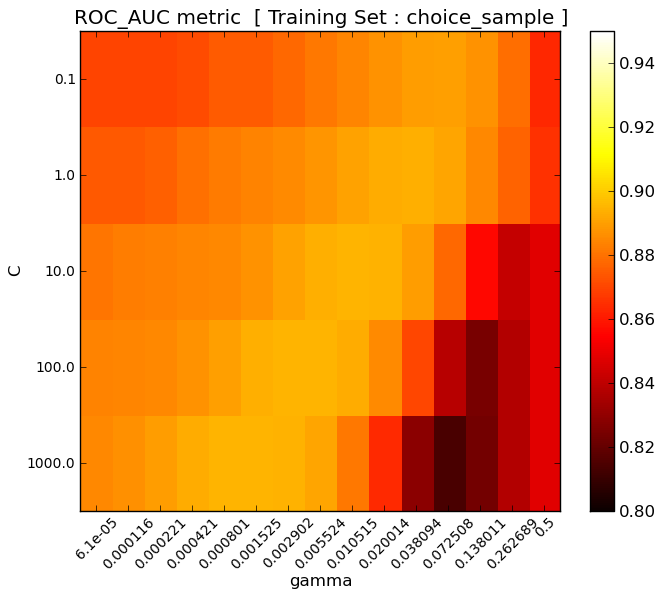
\includegraphics[scale=0.5]{Images/ROC_AUC_choice_sample_grid2.png} 
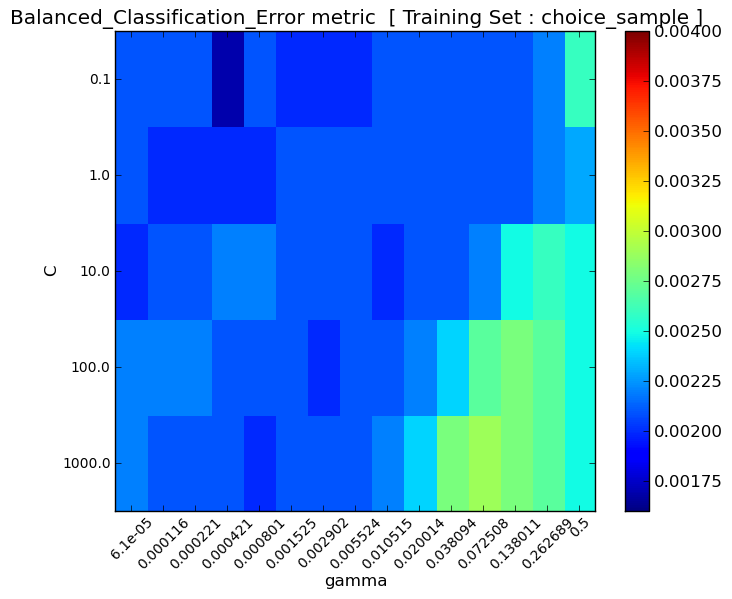
\includegraphics[scale=0.5]{Images/Balanced_Classification_Error_choice_sample_grid2.png} 
\caption{Grid search over base 10 grid of $C$ and $\gamma$ values. The uniform sample and the choice sample give very similar ROC and Balanced classification error patterns for values of $C$ and $\gamma$}
\label{metrics_grid2}
\end{figure*}

\subsection{AMS Performance}

The AMS performance over a range of thresholds is summarized in fig. \ref{AMSSVM}.

We choose 3 parameter combinations from the diagonal (see fig. \ref{metrics_grid2}) that gives the lowest balanced classification error.

\begin{figure}
\hspace{-0.3cm}
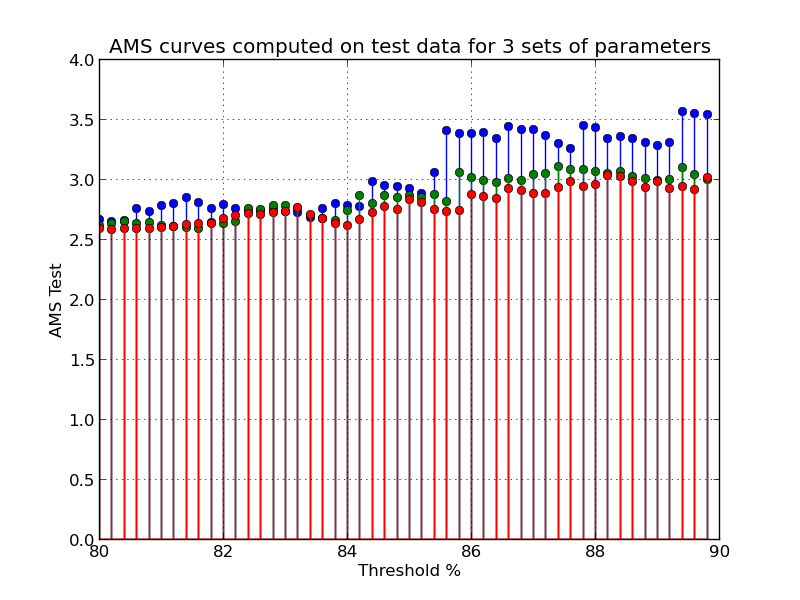
\includegraphics[scale=0.4]{Images/AMS_SVM_Optimum.png}
\caption{Optimized AMS curves for 3 sets of parameters in \ref{best}}
\label{AMSSVM}
\end{figure}

\begin{table}
\hspace{1.2cm}
\begin{tabular}{l|l|l}
Parameter $\Rightarrow$ & C & $\gamma$  \\
\toprule
Blue & 10 &  0.01\\
Green & 100 & 0.0004\\
Red &  1000  & 0.0001 \\
\end{tabular}
\caption{Best parameters for SVM}
\label{best}
\end{table}

Again, we observe the sensitivity of the AMS metric to the choice of threshold and further, more than one parameter combination of $C$ and $\gamma$ give high AMS values. 

\subsubsection{AMS without $CakeA$ Feature}

Figure \ref{AMSNoA} summarizes the performance of the AMS on the TEST set with the optimized SVM parameters (Blue) but without the analytically computed $CakeA$ feature.

\begin{figure}
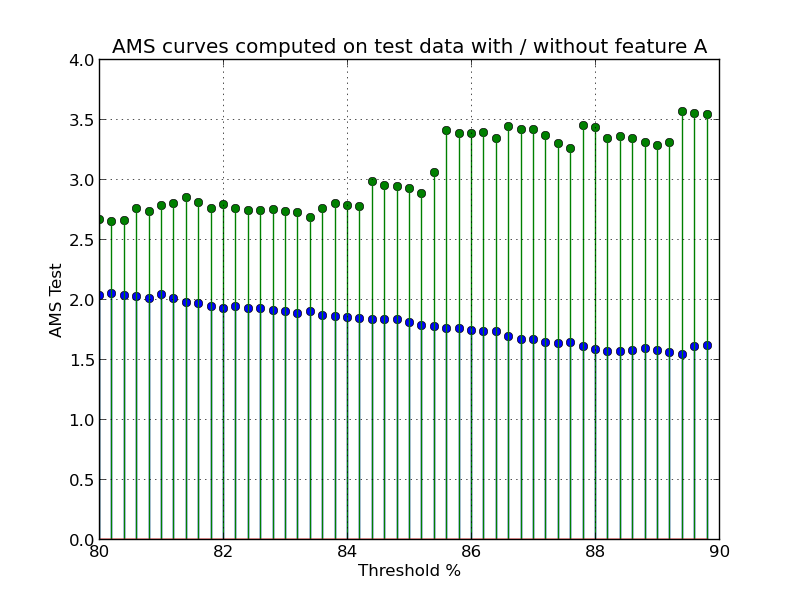
\includegraphics[scale=0.4]{Images/AMS_NO_A.png}
\caption{AMS without feature A}
\label{AMSNoA}
\end{figure}

It is hard to quantify in exact terms but there does seem to be a significant improvement in the AMS score across the board with the inclusion of $CakeA$. 


\subsection{Computational Performance}

An important advantage of using SVMs is that it is a convex optimization problem that can be successfully solved by quadratic programming techniques. The \texttt{sklearn} package used to build the classifier uses the \textit{Sequential Minimization Optimization} (SMO) algorithm which was developed by John Platt (1998) at Microsoft Research \cite{SMO}. SMO is an iterative algorithm that works by breaking the problem into a series of small sub problems which are then solved analytically. SMO essentially skips the quadratic programming part altogether. It uses heuristics to choose a pair of Lagrange multipliers to be considered at each step. In terms of computational complexity the SMO algorithm yields anywhere between linear and quadratic complexity depending on the problem. This is an improvement from the traditional SVM training complexity which is $O(n^3)$ in the number of  training data points. 

The table \ref{cp} below summarizes some of the runtime metrics of the SVM algorithm fitted to the Higgs dataset. 

\begin{table}
\hspace{-1cm}
\begin{tabular}{l|l}
Metrics & Values  \\
\toprule
Size of grid (for search) & $15 \times 5 = 75$ combinations of (C,$\gamma$) \\
No. of training samples & 10000 \\
Cross-validation (CV) & 3-fold  \\
Number of fits & 225 fits (75 $\times$ 3) \\
CV runtime &  $~$4.8 minutes\\
Runtime of 1 fit &  11 seconds  \\
\end{tabular}
\caption{SVM Computational Performance}
\label{cp}
\end{table}

\subsubsection{Benchmarking Results}

The highest score out of the 1785 published AMS scores on the Higgs dataset is 3.80. Out of the wide variety of models used on the datset, the most popular approaches were neural networks and boosted decision trees. Further, ensemble models which harmonize the output of several underlying models were also quite popular among participants. There were no solutions in the top $20\%$ of the solutions which used SVMs for the classification task. 

This paper contributes a prototype model whereby the use of SVMs has been demonstrated on the binary classification task. With carefully tuned parameters it achieves scores of well above 3.2 (this was the score on the benchmark algorithm provided by ATLAS, it uses boosted decision tree model). The Higgs dataset is challenging not only because of the overlapping and skewed class distributions but also because the custom objective function $-$ the AMS is an unusual one. Direct optimization of the AMS is difficult because the value of the metric is susceptible to jumps, this creates a new problem of trying to find metrics that are closely aligned with the AMS.   

\begin{figure}
\hspace{-0.7cm}
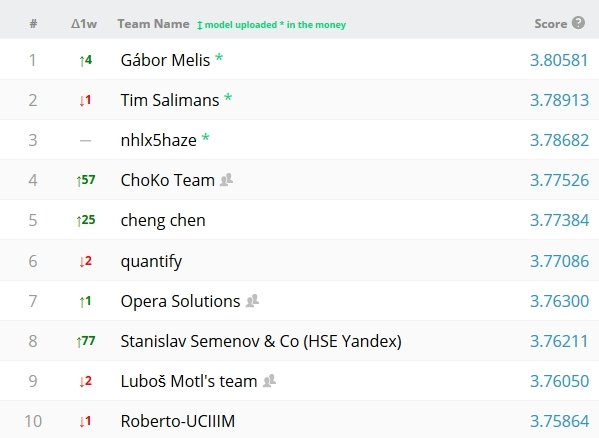
\includegraphics[scale=0.4]{Images/leaderboard_final.jpg} \\
\caption{Current top scores for machine learning performance on the Higgs dataset measured in terms of the AMS}
\end{figure}
\section{Conclusion and Further work}

In this paper we followed the approach of carefully condensing the size of the dataset provided for training. This proved to be a worthwhile trade-off between compute time and    
test performance. It is very interesting to observe how training on less than $10\%$ of the original dataset can yield viable classifiers with accuracies higher than $80\%$. 

The focus of this paper was to demonstrate the usage of SVMs on the Higgs classification problem. There are many ways in which this prototype can be enhanced and fine-tuned to the specific problem. Some of the ideas are suggested below, 

\begin{enumerate}
\item Online SVM which relies on incremental learning where training data is provided one example at a time rather than batch mode in which all samples are provided at once is a classical approach to training SVMs on large datasets. 
\item The dimensionality of the Higgs dataset is not a bottleneck to training however computational speed-up in the factor of 5 to 20 can be achieved by minimizing the number of redundant features in the dataset. There are several formal approaches that can be tried, PCA for instance has been traditionally very successful in enriching high dimensional problems with information about the importance of each feature through principal component scores.
\item Using analytical physics features (like $CakeA$) to guide the algorithms at the time of training can prove paramount to maximizing the objective.  
\end{enumerate}

\label{conclusion}

\section*{Acknowledgements}

I acknowledge the assistance of my supervisor Dr. Anita Faul who provided the intuition for the sampling idea and Dr. Christopher Lester who helped with understanding the physics goal of the problem. 

\section*{References}
\bibliography{References_SVM} 
\bibliographystyle{elsart-num-names.bst}

\appendix

\section{Invariant mass principle}

\label{AppA}

This section is based on \cite{RM}.

A fundamental equation of special relativity is, $$ E^2 = p^2c^2 + m^2c^4 $$ where $E$ is the energy of the particle, $p$ is its momentum, $m$ is the mass and $c$ is the speed of light. When a particle is at rest its momentum is 0, this gives us Einstein's mass-energy equivalence, $E = mc^2$.  Using the units GeV for Energy, GeV$/c$ for momentum and GeV$/c^2$ for mass we get the equivalence,  $$E^2 = p^2 + m^2 $$ The papers published in the ATLAS and CMS experiment use the notation GeV for mass, energy and momentum. We will follow the same convention.

The momentum $p$ of a particle is actually a 3-dimensional vector $\overrightarrow{p} = (p_{x}, p_{y}, p_{z})$ stating the particle's momentum in 3 directions in 3-d space. For a particle with non-zero mass the momentum of a particle is $\overrightarrow{p} = m\overrightarrow{v}$ where $\overrightarrow{v}$ is the 3-dimensional velocity and $m$ is the mass. The 4-momentum of a particle is defined as $(p_{x}, p_{y}, p_{z}, E)$. This defines the full kinematics of a particle as if we know the particle's momentum and energy we can compute its mass using the relation, $$ m = \sqrt{E^2 - p^2} $$

Similarly, if we know any two quantities out of momentum, mass and energy we can compute the third deterministically by equations of special relativity specified above. 

The mass of a particle is an intrinsic property of a particle, further by the law of conservation of energy and momentum the mass of a particle is equivalent to the mass of its decayed products each of which can be represented by their 4-momentum. For example, a particle $\chi$ decays into two final state particles $a$ and $b$ whose kinematics are captured in the detector. By conservation of energy and momentum, $$E_{\chi} = E_{a} + E_{b}$$ $$\overrightarrow{p_{\chi}} = \overrightarrow{p_{a}} + \overrightarrow{p_{b}}$$

The sum of energies and momenta of particles $a$ and $b$ should resolve to give the energy and momenta of the parent particle. The mass of the parent particle is then calculated as, $$ m_{\chi} = \sqrt{E_{\chi}^2 - p_{\chi}^2} $$ 

This is the \textit{invariant mass principle} in classical mechanics. It holds for all particles including the Higgs boson and can be generalised to more than two final states and holds in every intermediate stage of decay.   


\section{Physical meaning of Features}

\label{Pfeatures}

In the 3-d reference frame, we assume the z-axis to be the horizontal beam line. Transverse quantities are quantities projected on the plane perpendicular to the beam line, this is the $x-y$ plane. We stated earlier that the primary ingredients needed to compute the characteristics of the parent particle are the 4-momentum vectors $(p_{x}, p_{y}, p_{z}, E)$ for each of the decay products. The primary features in our dataset are quantities derived from the raw 4-momentum coordinates. These physical quantities constructed by ATLAS physicsts capture properties of the decay channel most critical to the inference of the parent particle. Below we describe these quantities which are used as features in our problem. The dataset comprises these quantities for each particle in the final-state of the collision. \cite{RM}

\textbf{Pseudorapidity ($\eta$)} : This describes the angle of the particle relative to the beam axis. It is defined as, $$ \eta = -ln [\tan(\theta/2)]$$ where $\theta$ denotes the angle between the particle and the positive direction of the beam axis. The diagram below depicts the concept, 

\begin{center}
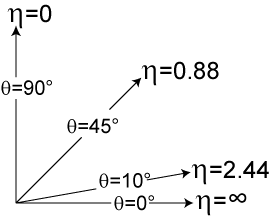
\includegraphics[scale=0.7]{Images/Pseudorapidity2.png}
\end{center}

$\eta = 0 $ corresponds to a particle in the $x-y$ plane perpendicular to the beam line, $\eta = +\infty$ corresponds to a particle travelling along the z-axis in the positive direction and $\eta = -\infty$ denotes travel in the opposite direction. Particles with high $\eta$ are usually lost and not captured by the detector. 

Particles can be identified in the range $\eta \in [-2.5 +2.5]$, for $|\eta| \in [2.5,5]$, their momentum can be measured but the particle cannot be identified. Particles with $|\eta| > 5$ escape detection all together \cite{RM}. 

\textbf{Azimuth Angle ($\phi$)} : Decay particles shoot out from the vertex of the collision which lies on the z-axis. The vector from the vertex to the particle is projected onto the transverse plane ($x-y$), the angle between the projected vector and the $x$-axis is the azimuth angle. 

\textbf{Transverse momentum  ($t$)} : The transverse momentum can be defined as the momentum that materializes in the $x-y$ plane perpendicular to the beam axis. A hard collision event is characterized by a high $t$, while proton collisions that result from protons brushing against each other leave decay particles not too far from the beam axis resulting in a small $t$. 

The transverse momentum is computed as, $$ t = \sqrt{p_{x}^2 + p_{y}^2}$$.

\end{document}

